\documentclass[xcolor={dvipsnames}, notheorems]{beamer}

\mode<presentation> {


%\usetheme{default}
%\usetheme{AnnArbor},
%\usetheme{Antibes} 
%\usetheme{Bergen}
%\usetheme{Berkeley}
% \usetheme{Berlin}
%\usetheme{Boadilla}
%\usetheme{CambridgeUS}
%\usetheme{Copenhagen}
%\usetheme{Darmstadt}
%\usetheme{Dresden}
%\usetheme{Frankfurt}
%\usetheme{Goettingen}
%\usetheme{Hannover}
%\usetheme{Ilmenau}
%\usetheme{JuanLesPins}
%\usetheme{Luebeck}
\usetheme{Madrid}
%\usetheme{Malmoe}
%\usetheme{Marburg}
%\usetheme{Montpellier}
%\usetheme{PaloAlto}
%\usetheme{Pittsburgh}
%\usetheme{Rochester}
%\usetheme{Singapore}
%\usetheme{Szeged}
%\usetheme{Warsaw}
%\usecolortheme{albatross}
%\usecolortheme{beaver}
%\usecolortheme{beetle}
%\usecolortheme{crane}
%\usecolortheme{dolphin}
%\usecolortheme{dove}
%\usecolortheme{fly}
%\usecolortheme{lily}
%\usecolortheme{orchid}
%\usecolortheme{rose}
%\usecolortheme{seagull}
%\usecolortheme{seahorse}
%\usecolortheme{whale}
%\usecolortheme{wolverine}

%\setbeamertemplate{footline} % To remove the footer line in all slides uncomment this line
%\setbeamertemplate{footline}[page number] % To replace the footer line in all slides with a simple slide count uncomment this line

%\setbeamertemplate{navigation symbols}{} % To remove the navigation symbols from the bottom of all slides uncomment this line
}

\usepackage{graphicx} % Allows including images
\graphicspath{{/Users/justindoty/Documents/Research/Dissertation/Production_QR_Proxy/Code/Figures/}}
% \graphicspath{{/Users/justindoty/Desktop/QPF/Figures/}}
% \graphicspath{{/Users/suysong/Dropbox/AAA_Song/Research/JustinDoty/QuantileProductionFunction/text/Figures/}}
\usepackage{booktabs} % Allows the use of \toprule, \midrule and \bottomrule in tables
\usepackage{amsmath}
\usepackage{amssymb}
\usepackage{amstext}
\usepackage{amsthm}
\usepackage{mathrsfs}
\usepackage{caption}
\usepackage{subcaption}
\usepackage{bbm} 
\setbeamertemplate{theorems}[numbered]
\setbeamertemplate{caption}[numbered]
\theoremstyle{plain}
\newtheorem{assump}{Assumption}
\newtheorem{definition}{Definition}
\newtheorem{lemma}{Lemma}
\newtheorem{corollary}{Corollary}
\newtheorem{theorem}{Theorem}
\newcommand{\indep}{\perp \!\!\! \perp}
\usepackage[natbib=true,style=authoryear,backend=bibtex,useprefix=true]{biblatex}
\addbibresource{/Users/justindoty/Documents/Research/Dissertation/Production_QR_Proxy/Code/Text/references.bib}


%------------------------------------------------------------------------------
%	TITLE PAGE
%------------------------------------------------------------------------------

\title[Quantile Production Functions]{Estimating Quantile Production Functions:\\
A Control Function Approach}

\author[Doty \& Song (2021)]{Justin Doty and Suyong Song} % 
\institute[]{University of Iowa} % Your institution as it will appear on the bottom of every slide, may be shorthand to save space
{

\medskip % Your email address
}
\date{\today} % Date, can be changed to a custom date

\begin{document}

\begin{frame}
\titlepage % Print the title page as the first slide
\end{frame}

%------------------------------------------------------------------------------
%	PRESENTATION SLIDES
%------------------------------------------------

\begin{frame}
\frametitle{Introduction}
\begin{itemize}
\item Production function estimation is an ongoing and historical research topic
\item Links inputs (capital goods, labor, intermediate inputs, etc) to output
\item Estimates provide insights on how firm productivity changes over time and cross-sectional differences between firms
\item Most inputs and output are observed (albeit with possible measurement error) in data such as manufacturing censuses or constructed from data from firm financial statements
\item Other inputs to production, such as managerial ability, are not observed in the data. 
\item This type of unobserved productivity influences how much inputs a firm uses in production
\item As such, if unobserved, biases OLS estimates. This is known as ``simultaneity bias''
\end{itemize}
\end{frame}


%---------------------------------------------------------------------------------

\begin{frame}
\frametitle{Control Function Approach}
\begin{itemize}
\item A popular approach to address simultaneity bias and other econometric issues is the control function approach
\item Introduce a policy function such as investment \citep{Olley1996} (OP), or an intermediate input \citep{Levinsohn2003} (LP) or \citep{Ackerberg2015} (ACF)
\item If the policy functions depend only on current state variables (e.g. capital and productivity) under a monotonicity restriction, they can be inverted to proxy for the unobserved productivity component
\item  Computationally simple and has been used in numerous applied papers to obtain consistent estimates of output elasticities, total factor productivity, markups, etc.
\item Some issues still remain: identification issues related to model specification, measurement error and other unobservables
\end{itemize}
\end{frame}


%------------------------------------------------------------------------------

\begin{frame}
\frametitle{Control Function Approach}
\begin{itemize}
\item Review of the ACF procedure for estimating a \textit{value-added} production function (in logs):
\begin{equation}
y_{it}=\beta_{k}k_{it}+\beta_{l}l_{it}+\omega_{it}+\varepsilon_{it},
\end{equation}
\item $y_{it}$ is value-added output for firm $i$ and time $t$
\item $l_{it}$ denotes labor input
\item $k_{it}$ denotes capital input
\item $\omega_{it}$ is unobserved productivity
\item $\varepsilon_{it}$ denotes an independent and identically distributed (i.i.d)  shock to production
\item The constant $\beta_{0}$ is omitted since it is not separately identified from the mean of productivity.  
\end{itemize}
\end{frame}
%---------------------------------------------------------------------------------
\begin{frame}
\frametitle{Control Function Approach}
\begin{itemize}
\item ACF introduces an intermediate input demand function defined as
\begin{equation}
m_{it}=m_{t}(k_{it}, l_{it}, \omega_{it})
\end{equation} 
\item The function $m$ is assumed to be strictly increasing in $\omega_{it}$ for all $k_{it}$ and $l_{it}$. 
\item Productivity can then be expressed as
\begin{equation}
\omega_{it}=m_{t}^{-1}(k_{it}, l_{it}, m_{it})
\end{equation}
\item Substituting this equation into the production function
\begin{equation}
y_{it}=\beta_{k}k_{it}+\beta_{l}l_{it}+m^{-1}_{t}(k_{it}, l_{it}, m_{it})+\varepsilon_{it}=\Phi_{t}(k_{it}, l_{it}, m_{it})+\varepsilon_{it}.
\end{equation}
\item The function, $\Phi_{t}(k_{it}, l_{it}, m_{it})$, is identified by the following first stage moment restriction
\begin{equation}
\mathbb{E}[\varepsilon_{it}|\mathcal{I}_{it}]=0
\end{equation}
\item $\mathcal{I}_{it}$ denotes the firm's information at time $t$. 
\item The first stage estimate of $\Phi_{t}$ can be obtained by a local linear regression or a polynomial regression in $(k_{it}, l_{it}, m_{it}).$
\end{itemize}
\end{frame}
%------------------------------------------------------------------------------------

\begin{frame}
\frametitle{Control Function Approach}
\begin{itemize}
\item For the second stage, assume that productivity follows an AR(1) process given by
\begin{equation}
\omega_{it}=\mathbb{E}[\omega_{it}|\omega_{it-1}]+\xi_{it}=\rho\omega_{it-1}+\xi_{it},
\end{equation}
\item $\xi_{it}$ denotes an innovation to productivity which satisfies $\mathbb{E}[\xi_{it}|\mathcal{I}_{it-1}]=0$.
\item Plugging into the production function gives
\begin{equation*}
\begin{split}
y_{it}&=\beta_{k}k_{it}+\beta_{l}l_{it}+\rho\omega_{it-1}+\xi_{it}+\varepsilon_{it}\\
&=\beta_{k}k_{it}+\beta_{l}l_{it}+\rho(\Phi_{t-1}(k_{it-1}, l_{it-1}, m_{it-1})-\beta_{k}k_{it-1}-\beta_{l}l_{it-1})+\xi_{it}+\varepsilon_{it}.
\end{split}
\end{equation*}
\item The production function parameters $\beta_{k}, \beta_{l}$ and $\rho$ are identified from the moment restrictions given by
\begin{equation}\label{2ndstagemoment}
\mathbb{E}[\xi_{it}+\varepsilon_{it}|\mathcal{I}_{it-1}]=0.
\end{equation}
\item Estimation of the second stage coefficients proceeds by plugging in first stage estimates $\hat{\Phi}_{t-1}$ and forming a Generalized Method of Moments (GMM) criterion function.
\end{itemize}
\end{frame}

%------------------------------------------------------------------------------------

\begin{frame}
\frametitle{Control Function Approach}
\begin{itemize}
\item These estimates only provide a picture of the conditional mean of firm output
\item Quantile regression offers robust estimates to outliers in the data
\item Not straightforward to estimate production functions with endogenous inputs and heterogeneous coefficients
\item The conditional mean restrictions in ACF to do not extend naturally to conditional quantile restrictions with multiple unobservables
\item Expectation operators are linear whereas quantile operators are not
\item Similar issues are encountered in the quantile panel data literature
\item  First to address simultaneity and quantiles in the production function literature
\item Propose an easy-to-implement estimator motivated by our identification argument which is consistent and asymptotically normal
\end{itemize}
\end{frame}

%------------------------------------------------------------------------------------

\begin{frame}
\frametitle{Random Coefficient Production Function}
\begin{itemize}
\item A Skorohod representation for a firm's \textit{value-added} production function:
\begin{equation} \label{pfrc}
    y_{it}=\beta_{k}(\eta_{it})k_{it}+\beta_{l}(\eta_{it})l_{it}+\omega_{it}, \quad \text{where}\quad \eta_{it}\sim U(0,1),
\end{equation}
\item $Q_{\tau}(y_{it}|\mathcal{I}_{it})$ is the conditional $\tau$-th quantile of $y_{it}$ given the information set $\mathcal{I}_{it}$ for $\tau\in(0,1)$.
\item Skorohod representation assumes that the unobserved heterogeneity enters through the rank of a firm on the conditional output distribution
\item $\eta_{it}$ is a technology shock, not to be confused with ex-post shock $\varepsilon_{it}$
\item Productivity $\omega_{it}$ is additively separable and does not depend on $\eta_{it}$
\item $\omega_{it}$ is only a location-shift of the conditional output distribution
\item Assume the constant in the production function does not vary over $\tau$ and subsume it into the productivity term
\end{itemize}
\end{frame}

%------------------------------------------------------------------------------------

\begin{frame}
\frametitle{Random Coefficient Production Function}
\begin{itemize}
\item  A value-added specification in equation \eqref{pfrc} is non-trivial
\item Objects recovered from a value-added model such as the output elasticities and TFP can only be mapped to its gross-output counterpart under special structural production function (Leontief value-added)
\item In this case, a Leontief value-added production function in this framework could be written as
\begin{equation*}
y_{it}=\min\{\beta_{k}(\eta_{it})k_{it}+\beta_{l}(\eta_{it})l_{it}+\omega_{it}, \beta_{m}+m_{it}\},
\end{equation*}
\item Thanks to the equivariance properties of quantiles we have
\begin{equation*} 
Q_{\tau}(y_{it}|\mathcal{I}_{it})=\min\{\beta_{k}(\tau)k_{it}+\beta_{l}(\tau)l_{it}+\omega_{it}, \beta_{m}+m_{it}\},
\end{equation*}
\item The conditional quantile of a structural value-added production function could be written as
\begin{equation*}
Q_{\tau}(y_{it}|\mathcal{I}_{it})=\beta_{k}(\tau)k_{it}+\beta_{l}(\tau)l_{it}+\omega_{it},
\end{equation*}
\item This corresponds directly to the conditional quantile of Equation \eqref{pfrc}
\end{itemize}
\end{frame}

%------------------------------------------------------------------------------------

\begin{frame}
\frametitle{Quantiles and Production Risk}
\begin{itemize}
\item  What factors contribute to dispersion in the conditional output distribution through rank of $\eta_{it}$?
\item Consider the location-scale model as a special case of \eqref{pfrc}
\begin{equation} \label{locationscale}
    y_{it}=\beta_{k}k_{it}+\beta_{l}l_{it}+\omega_{it}+(\mu_{k}k_{it}+\mu_{l}l_{it})\eta_{it},
\end{equation}
\item The $\tau$-th conditional quantile of $y_{it}$ is given by
\begin{equation}
Q_{\tau}(y_{it}|\mathcal{I}_{it})=\beta_{k}k_{it}+\beta_{l}l_{it}+\omega_{it}+(\mu_{k}k_{it}+\mu_{l}l_{it})F^{-1}(\tau),
\end{equation}
\item $F^{-1}(\tau)$ is the quantile function of production shocks $\eta_{it}$
\item Inputs chosen by the firm have some control over the risk of production
\item  \cite{Just1978,Just1979} consider a specification that allowed firm's inputs to both increase or decrease the marginal variability of final output
\end{itemize}
\end{frame}

%------------------------------------------------------------------------------------

\begin{frame}
\frametitle{Quantiles and Production Risk}
\begin{itemize}
\item How to extend this idea to the entire distribution of output? 
\item Requires reformulating how firms form beliefs about uncertainty in profits due to production risk
\item Instead of rational expectations framework, could we allow firms to have varying risk preferences and use a quantile profit maximization framework?
\item Different managers may choose different optimal expenditure on inputs to maximize profits in the presence of production risk
\item A short list of papers have considered quantile utility maximization such as \cite{Manski1988}, \cite{ROSTEK2009}, \cite{Chambers2007}, and \cite{Bhattacharya2009}
\item For dynamic problems, for example, investment decisions, \cite{Castro2019} may be applicable
\item Difficult to incorporate this theory into testable econometric models
\item Leave as future research agenda
\end{itemize}
\end{frame}

%------------------------------------------------------------------------------------

\begin{frame}
\frametitle{Quantiles and Frontier Models}
\begin{itemize}
\item The model presented here is also related to the stochastic frontier analysis (SFA) literature
\item A SFA model of production proposed by \cite{Aigner1977} introduces statistical error into a frontier model
\item Frontier models assume that firms deviate from an optimal frontier of production
\item The SFA model is typically written as
\begin{equation}
y_{i}=f(x_{i}, \beta)+\varepsilon_{i},
\end{equation}
\item $\varepsilon_{i}=\eta_{i}-u_{i}$, $x_{i}$ are inputs to production and $\beta$ are the parameters
\item The error term $\eta_{i}$ denotes the statistical noise in the model such as measurement error
\item $u_{it}$ represents one-sided deviations from the production frontier
\item Estimates of $\beta$ are typically obtained using maximum likelihood which requires strong distributional assumptions on the error terms
\end{itemize}
\end{frame}

%------------------------------------------------------------------------------------

\begin{frame}
\frametitle{Quantiles and Frontier Models}
\begin{itemize}
\item Quantile regression is a natural candidate for obtaining an estimate of the efficient frontier
\item \cite{Aragon2005} interprets production functions as being from a continuous interval $\tau\in[0,1]$ where $\tau\rightarrow 1$ converges to the efficient frontier
\item Difficulty in choosing which quantile to estimate as the frontier
\item Inference on extremal quantiles is difficult \citep{Chernozhukov2005a}
\item Statistical noise is also an issue since predicted error is composite of the technical inefficiency and noise
\item Other econometric issues, such as endogeneity of input choices with respect to inefficiency are difficult to incorporate in this framework
\item It is possible the model proposed in this paper could be applied here
\end{itemize}
\end{frame}

%------------------------------------------------------------------------------------

\begin{frame}
\frametitle{Identification}
\begin{itemize}
\item Show that the model presented in Equation \eqref{pfrc} is non-parametrically identified
\item Results can also be applied to other production functions such as translog, provided that productivity is additively separable
\item Let $\varepsilon_{it}=k_{it}[\beta_{k}(\eta_{it})-\beta^{\mu}_{k}]+l_{it}[\beta_{l}(\eta_{it})-\beta^{\mu}_{l}]$
\item A conditional mean equation for \eqref{pfrc} can be written as
\begin{equation}\label{meanversion}
y_{it}=\beta_{k}^{\mu}k_{it}+\beta_{l}^{\mu}l_{it}+\omega_{it}+\varepsilon_{it},
\end{equation}
\item Here, $\mathbbm{E}[\varepsilon_{it}|\mathcal{I}_{it}]=0$
\item The production function coefficients $\boldsymbol{\beta}(\tau)=(\beta_{k}(\tau), \beta_{l}(\tau))$ are non-parametrically identified with $T=2$ under conditional independence assumptions and other mild regularity conditions
\end{itemize}
\end{frame}

%------------------------------------------------------------------------------------

\begin{frame}
\frametitle{Identification}
\begin{itemize}
\item For ease of notation let $x_{it}=(k_{it}, l_{it}), x_{it+1}=(k_{it+1}, l_{it+1})$, and $x_{i}=(x_{it}, x_{it+1})$
\item Let $Z_{it}=\beta_{k}(\eta_{it})k_{it}+\beta_{l}(\eta_{ti})l_{it}$
\item For any random variable $X$ and $\rho\neq 0$, let $\tilde{X}=X/\rho$
\item Two consecutive period of output can be written as $y_{it}=Z_{it}+\omega_{it}$ and $y_{it+1}=Z_{it+1}+\omega_{it+1}$
\item  Assume a linear AR(1) process for productivity, $\omega_{it+1}=\rho\omega_{it}+\xi_{it+1}$
\item Plugging into second period observation equation gives $\tilde{y}_{it+1}=y_{it+1}/\rho=\tilde{Z}_{it+1}+\tilde{\xi}_{it+1}+\omega_{it}$
\item So there are two repeated measures of productivity
\begin{equation} \label{repeatedmeas}
\begin{split}
&y_{it}=Z_{it}+\omega_{it}\\
&\tilde{y}_{it+1}=\tilde{Z}_{it+1}+\tilde{\xi}_{it+1}+\omega_{it}.
\end{split}
\end{equation}
\end{itemize}
\end{frame}

%------------------------------------------------------------------------------------

\begin{frame}
\frametitle{Identification}
\begin{itemize}
\item Goal is identification of the conditional quantile
\begin{equation*}
Q_{\tau}(Z_{it}|x_{i})=x_{it}\boldsymbol\beta(\tau),
\end{equation*}
which can be identified if the conditional distribution function
\begin{equation}\label{CDF}
F_{Z_{it}|x_{i}}(Z_{it}|x_{i})=\frac{1}{2}-\underset{\upsilon\rightarrow \infty}{\operatorname{lim}}\int_{-\upsilon}^{\upsilon}\frac{e^{-\mathrm{i}sZ_{it}}}{2\pi \mathrm{i}s}\phi_{Z_{it}|x_{i}}(s|x_{i})ds,
\end{equation}
is identified
\item Since the quantile function is the inverse of the CDF, this implies identification of the conditional quantiles
\item Identification relies on the conditional characteristic functions $\phi_{Z_{it}|x_{i}}(s|x_{i})$ being identified
\end{itemize}
\end{frame}

%------------------------------------------------------------------------------------

\begin{frame}
\frametitle{Identification}
\begin{itemize}
\item Utilize conditional deconvolution arguments to identify this conditional characteristic functions up to an unknown location, $\mathbbm{E}[\omega_{it}|x_{i}]$
\item Similar ideas have been used in panel data models such as \cite{Neumann2007} and \cite{evdo2010}
\item Identification of the location relies on identification of $\boldsymbol{\beta}^{\mu}=(\beta_{k}^{\mu}, \beta_{l}^{\mu})$ from Equation \eqref{meanversion} and the parameter $\rho$
\item Similar to ACF, we show that these parameters are identified by the moment restriction $\mathbbm{E}[\xi_{it}+\varepsilon_{it}|\mathcal{I}_{it-1}]=0$ from Equation \eqref{2ndstagemoment}
\item Once this is established, the characteristic functions can be identified using $T=2$ firm-year observations.
\end{itemize}
\end{frame}

%------------------------------------------------------------------------------------

\begin{frame}
\frametitle{Identification}
\begin{assump}\label{idpart1}
\begin{itemize}
    \item Random Sample: The random variables $(y_{i}, Z_{i}, \omega_{i})_{i=1}^{N}$ are independently and identically distributed and $T=2$.
    \item Conditional Independence: (i) $f_{Z_{it}|Z_{it+1}, \xi_{it+1}, \omega_{it}, x_{i}}(Z_{it}|Z_{it+1}, \xi_{it+1}, \omega_{it}, x_{i})=f_{Z_{it}|x_{i}}(Z_{it}|x_{i})$, (ii) $f_{Z_{it+1}|\omega_{it+1}, x_{i}}(Z_{it+1}|\omega_{it+1}, x_{i})=f_{Z_{it+1}|x_{i}}(Z_{it+1}|x_{i})$,  and (iii) $f_{\xi_{it+1}|\omega_{it}, x_{i}}(\xi_{it+1}|\omega_{it}, x_{i})=f_{\xi_{it+1}|x_{i}}(\xi_{it+1}|x_{i})$.
    \item Characteristic Functions: The conditional characteristic functions $\phi_{Z_{it}|x_{i}}(s|x_{i})$ and $\phi_{\omega_{it}|x_{i}}(s|x_{i})$ do not vanish $\forall t\in\{1,\dots,T\}$ and $\phi_{\xi_{it}|x_{i}}(s|x_{i})$  does not vanish, $\forall t\in\{2,\dots,T\}$.
    \item Quantiles: $\eta_{it}\indep (x_{it}, \omega_{it})$ where $\eta_{it}\sim U(0,1)$ and $Z_{it}$ is strictly increasing in $\eta_{it}$.
\end{itemize}
\end{assump}
\end{frame}

%------------------------------------------------------------------------------------

\begin{frame}
\frametitle{Identification}
\small
\begin{assump}\label{idpart2}
\begin{itemize}
    \item Information Set: $\mathcal{I}_{it}$ only includes current and past productivity shocks.
    \item Productivity: Productivity follows $\omega_{it}=\rho\omega_{it-1}+\xi_{it}$, where $\xi_{it}$ is a shock that satisfies $\mathbbm{E}[\xi_{it}|\mathcal{I}_{it-1}]=0$
    \item Timing of  Input Choices: Firms accumulate capital according to
    \begin{equation*}
    K_{it}=\kappa(K_{it-1}, I_{it-1}).
    \end{equation*}
    \item Scalar Unobservable: Firm's intermediate input demand is given by
    \begin{equation*}
    m_{it}=m_{t}(k_{it}, l_{it}, \omega_{it}).
    \end{equation*}
    \item Strict Monotonicity: $m_{t}(k_{it}, l_{it}, \omega_{it})$ is strictly increasing in $\omega_{it}$.
    \item Identification: There exists a neighborhood of $(\boldsymbol{\beta}^{\mu}, \rho)$ such that  $(\boldsymbol{\beta}^{\mu}, \rho)$ is the unique solution to Equation \eqref{2ndstagemoment}.
\end{itemize}
\end{assump}
\end{frame}

%------------------------------------------------------------------------------------

\begin{frame}
\frametitle{Identification}
\begin{itemize}
\item Assumption \ref{idpart1}(a) places restrictions on the data generating process
\item Assumption \ref{idpart1}(b)(i) implies that $\eta_{it}$ is independent of $\eta_{it+1}$, $\xi_{it+1}$ and $\omega_{it}$ conditional on $x_{i}$
\item Assumption \ref{idpart1}(b)(ii) implies that $\eta_{it+1}$ is independent of $\omega_{it+1}$ conditional on $x_{i}$
\item Assumption \ref{idpart1}(b)(iii) implies $\xi_{it+1}$ is independent of $\omega_{it}$ conditional on $x_{i}$
\item Assumption \ref{idpart1}(c) are mild technical conditions on characteristic functions
\item Assumption \ref{idpart2} is a modification of the ACF assumptions used to prove identification of $\mathbbm{E}[\omega_{it}|x_{i}]$
\end{itemize}
\end{frame}

%------------------------------------------------------------------------------------

\begin{frame}
\frametitle{Identification}
\begin{theorem} \label{idtheorem}
Under Assumptions \ref{idpart1} and \ref{idpart2}, the location parameters $\boldsymbol{\beta}^{\mu}$ and $\rho$, the function $\boldsymbol{\beta}(\tau)$ for each $\tau\in(0,1)$ and the distribution of productivity are identified.
\end{theorem}
\end{frame}

%------------------------------------------------------------------------------------

\begin{frame}
\frametitle{Econometric Procedure}
\begin{itemize}
    \item Estimation can proceed by constructing sample moments based on the conditional characteristic functions
    \item Then these estimates can be plugged into \eqref{CDF} and the conditional quantiles can constructed from the inverse relationship between CDF and quantiles
    \item This approach would be computationally burdensome. Provide a simple estimator that is consistent and asymptotically normal
    \item Recall $\varepsilon_{it}=k_{it}[\beta_{k}(\eta_{it})-\beta^{\mu}_{k}]+l_{it}[\beta_{l}(\eta_{it})-\beta^{\mu}_{l}]$ 
    \item Here $(\beta_{k}^{\mu}, \beta_{l}^{\mu})=\boldsymbol{\beta}^{\mu}=\mathbbm{E}[\boldsymbol{\beta}(\eta_{it})]$ is the mean of the random coefficients
    \item The conditional mean version of the random coefficient production function is 
    \begin{equation}
    y_{it}=\beta_{k}^{\mu}k_{it}+\beta_{l}^{\mu}l_{it}+\omega_{it}+\varepsilon_{it},
    \end{equation}
    where $\mathbbm{E}[\varepsilon_{it}|\mathcal{I}_{it}]=0$
\end{itemize}
\end{frame}


%------------------------------------------------------------------------------------

\begin{frame}
\frametitle{Econometric Procedure}
\begin{block}{Estimation Procedure}
\begin{enumerate}
    \item Let $\hat{\beta}_{k}^{\mu}$ and $\hat{\beta}_{l}^{\mu}$ be consistent estimators of $\beta_{k}^{\mu}$ and $\beta_{l}^{\mu}$ from a value-added production function. Construct the estimator, $\hat{\omega}_{it}=\hat{\Phi}_{t}(k_{it}, l_{it}, m_{it})-\hat{\beta}^{\mu}_{k}k_{it}-\hat{\beta}^{\mu}_{l}l_{it}$, using these estimates.
    \item Let $\boldsymbol{\beta}(\tau)=(\beta_{k}(\tau), \beta_{l}(\tau))$ and $\hat{y}_{it}=y_{it}-\hat{\omega}_{it}$. For $\tau \in (0, 1)$, define the two-step estimator of $\boldsymbol{\beta}(\tau)$ as:
    \begin{equation*}
    \hat{\boldsymbol{\beta}}(\tau)=\underset{\boldsymbol{\beta}\in\mathcal{B}}{\operatorname{argmin}}\, \mathbbm{E}\big[\rho_{\tau}(\hat{y}_{it}-\beta_{k}k_{it}-\beta_{l}l_{it})\big],
    \end{equation*}
    where $\mathcal{B}$ is a compact and convex parameter space, $\rho_{\tau}(u)=u[\tau-\mathbbm{I}\{u<0\}]$, and $\mathbbm{I}\{\cdot\}$ denotes the indicator function.
\end{enumerate}
\end{block}
\end{frame}

%------------------------------------------------------------------------------------

\begin{frame}
\frametitle{Large Sample Properties}
\begin{itemize}
	\item The two-step estimator relies on an initial consistent estimator of productivity
	\item Standard errors from the estimator of the asymptotic covariance matrix include the variance from these estimate
	\item  The model falls under a class of generated dependent variables in quantile regression
	\item The main challenge of our approach is two-fold
	\begin{enumerate}
		\item the first stage is semi-parametric due to the non-parametric function, $\Phi_{t}(k_{it}, l_{it}, m_{it})$
		\item The finite parameters $\beta_{k}^{\mu}$ and $\beta_{l}^{\mu}$ and the asymptotic covariance matrix for $\beta_{k}^{\mu}$ and $\beta_{l}^{\mu}$ include the variance from estimating $\Phi_{t}(k_{it}, l_{it}, m_{it})$
	\end{enumerate}
	\item In the main text, it is shown that following \cite{Chernozhukov2005} the quantile regression estimates are consistent and asymptotically normal
\end{itemize}
\end{frame}

%------------------------------------------------------------------------------------

\begin{frame}
\frametitle{Large Sample Properties}
\begin{itemize}
	\item Estimation of the asymptotic covariance matrix is complicated in the two-step semi-parametric approach
	\item Need to estimate an influence function that is derived from ACF estimator
	\begin{equation*}
		\psi_{it}=
		\begin{pmatrix}
		\psi^{\theta}_{it}\\
		\psi^{\beta{\mu}}_{it}
		\end{pmatrix}
		=
		\begin{pmatrix}
		\Sigma_{z}^{-1}g_{1}(Z_{t};\theta)\\
		-(D_{\beta^{\mu}}\Sigma_{x}D_{\beta^{\mu}}^{'})^{-1}D_{\beta^{\mu}}\Sigma_{x}g_{2}(x; \beta^{\mu}, \theta)
		\end{pmatrix}.
	\end{equation*}
	\item Assumed that $\Sigma_{z}=\mathbbm{E}[\mu_{z}\mu_{z}^{'}]$ is non-singular with finite norm
	\item $g_{1}(Z_{t};\theta)=p^{k_{n}}(z_{it})\varepsilon_{it}$ from first stage
	\item $g_{2}(x; \beta^{\mu}, \theta)$ from second stage
	\item $\Sigma_{x}$ is a positive-definite weighting matrix
	\item $D_{\beta^{\mu}}=\frac{\partial}{\partial \beta^{\mu}}g_{2}(x; \beta^{\mu}, \theta)$
	\item Instead, nonparametric bootstrap is used for inference
\end{itemize}
\end{frame}

%------------------------------------------------------------------------------------

\begin{frame}
\frametitle{Monte Carlo Experiments}
\begin{itemize}
    \item A location-scale model for the production function is specified as
    \begin{equation} \label{simmodel}
    y_{it}=\beta_{k}k_{it}+\beta_{l}l_{it}+\omega_{it}+(\gamma_{k}k_{it}+\gamma_{l}l_{it})\eta_{it}
    \end{equation}
    where $\beta_{k}=0.4$ and $\beta_{l}=0.6$
    \item Replicate ACF simulations by sampling 1000 datasets consisting of 1000 firms
    \item Simulate optimal input choices for 100 time periods, using the last 10 periods for estimation
    \item Consider three different data generating processes (DGPs) for the scale parameters and the distribution of $\eta_{it}$
    \begin{enumerate}
        \item DGP 1: $\gamma_{k}=0.6$, $\gamma_{l}=-0.6$ and $\eta_{it}\sim N(0,\sigma_{\eta}^{2})$ where $\sigma_{\eta}^{2}=0.01$
        \item DGP2: $\gamma_{k}=0.4$, $\gamma_{l}=-0.4$ and $\eta_{it}\sim (\sqrt{3\sigma_{\eta}^{2}/5})t_{5}$
        \item DGP3: $\gamma_{k}=0.5$, $\gamma_{l}=-0.5$, and $\eta_{it}\sim Lognormal(0.15,\sigma_{\eta}^{2})$
    \end{enumerate}
    \item Productivity follows $\omega_{it}=\rho\omega_{it-1}+\xi_{it}$ where $\rho=0.7$
\end{itemize}
\end{frame}

%------------------------------------------------------------------------------------

\begin{frame}
\frametitle{Monte Carlo Results}
\resizebox{\linewidth}{!}{
\begin{tabular}{cccccccccc}
  \hline\hline & & & \multicolumn{2}{c}{DS} & & & \multicolumn{2}{c}{QR} \\ \cmidrule(lr){3-6} \cmidrule(lr){7-10} \\ & & \multicolumn{2}{c}{Capital} & \multicolumn{2}{c}{Labor} & \multicolumn{2}{c}{Capital} & \multicolumn{2}{c}{Labor} \\ \cmidrule(lr){3-4} \cmidrule(lr){5-6} \cmidrule(lr){7-8} \cmidrule(lr){9-10}DGP & $\tau$ & Bias & MSE & Bias & MSE & Bias & MSE & Bias & MSE \\ 
  \hline
  ACF 1 & 0.10 & -0.0099 & 0.0003 & 0.0129 & 0.0003 & 0.2881 & 0.0831 & -0.2941 & 0.0865 \\ 
   & 0.25 & -0.0035 & 0.0003 & 0.0045 & 0.0001 & 0.3115 & 0.0971 & -0.3175 & 0.1008 \\ 
   & 0.50 & -0.0010 & 0.0002 & 0.0000 & 0.0001 & 0.3380 & 0.1143 & -0.3440 & 0.1184 \\ 
   & 0.75 & 0.0025 & 0.0003 & -0.0035 & 0.0001 & 0.3645 & 0.1329 & -0.3715 & 0.1380 \\ 
   & 0.90 & 0.0089 & 0.0003 & -0.0119 & 0.0002 & 0.3889 & 0.1513 & -0.3949 & 0.1560 \\ 
  ACF 2 & 0.10 & -0.0057 & 0.0002 & 0.0087 & 0.0002 & 0.3053 & 0.0611 & -0.3103 & 0.0635 \\ 
   & 0.25 & -0.0015 & 0.0002 & 0.0025 & 0.0001 & 0.3225 & 0.0870 & -0.3285 & 0.0906 \\ 
   & 0.50 & 0.0000 & 0.0002 & 0.0000 & 0.0001 & 0.3390 & 0.1150 & -0.3450 & 0.1190 \\ 
   & 0.75 & 0.0025 & 0.0002 & -0.0025 & 0.0001 & 0.3555 & 0.1461 & -0.3615 & 0.1506 \\ 
   & 0.90 & 0.0067 & 0.0003 & -0.0077 & 0.0001 & 0.3727 & 0.1850 & -0.3787 & 0.1910 \\ 
  ACF 3 & 0.10 & -0.0043 & 0.0003 & 0.0043 & 0.0001 & 0.3067 & 0.0975 & -0.3127 & 0.1013 \\ 
   & 0.25 & -0.0015 & 0.0003 & 0.0015 & 0.0001 & 0.3145 & 0.0998 & -0.3205 & 0.1036 \\ 
   & 0.50 & -0.0006 & 0.0003 & 0.0006 & 0.0001 & 0.3294 & 0.1057 & -0.3354 & 0.1096 \\ 
   & 0.75 & 0.0019 & 0.0003 & -0.0029 & 0.0001 & 0.3519 & 0.1196 & -0.3579 & 0.1245 \\ 
   & 0.90 & 0.0097 & 0.0004 & -0.0137 & 0.0003 & 0.3817 & 0.1459 & -0.3877 & 0.1513 \\ 
   \hline
\end{tabular}}
\end{frame}

%------------------------------------------------------------------------------------

\begin{frame}
\frametitle{Monte Carlo Results}
\resizebox{\linewidth}{!}{
\begin{tabular}{cccccccccc}
  \hline\hline & & & \multicolumn{2}{c}{DS} & & & \multicolumn{2}{c}{QR} \\ \cmidrule(lr){3-6} \cmidrule(lr){7-10} \\ & & \multicolumn{2}{c}{Capital} & \multicolumn{2}{c}{Labor} & \multicolumn{2}{c}{Capital} & \multicolumn{2}{c}{Labor} \\ \cmidrule(lr){3-4} \cmidrule(lr){5-6} \cmidrule(lr){7-8} \cmidrule(lr){9-10}DGP & $\tau$ & Bias & MSE & Bias & MSE & Bias & MSE & Bias & MSE \\ 
  \hline
  LP 1 & 0.10 & -0.0149 & 0.0004 & 0.0199 & 0.0004 & 0.2691 & 0.0830 & -0.2771 & 0.0865 \\ 
   & 0.25 & -0.0045 & 0.0002 & 0.0065 & 0.0000 & 0.2905 & 0.0971 & -0.2975 & 0.1008 \\ 
   & 0.50 & 0.0010 & 0.0002 & 0.0000 & 0.0000 & 0.3140 & 0.1143 & -0.3210 & 0.1183 \\ 
   & 0.75 & 0.0065 & 0.0002 & -0.0065 & 0.0000 & 0.3375 & 0.1329 & -0.3445 & 0.1380 \\ 
   & 0.90 & 0.0169 & 0.0005 & -0.0199 & 0.0004 & 0.3589 & 0.1513 & -0.3659 & 0.1560 \\ 
  LP 2 & 0.10 & -0.0097 & 0.0003 & 0.0127 & 0.0002 & 0.2833 & 0.0610 & -0.2903 & 0.0635 \\ 
   & 0.25 & -0.0035 & 0.0002 & 0.0035 & 0.0000 & 0.2985 & 0.0870 & -0.3065 & 0.0905 \\ 
   & 0.50 & 0.0000 & 0.0002 & 0.0000 & 0.0000 & 0.3140 & 0.1149 & -0.3210 & 0.1190 \\ 
   & 0.75 & 0.0035 & 0.0002 & -0.0035 & 0.0000 & 0.3285 & 0.1460 & -0.3365 & 0.1506 \\ 
   & 0.90 & 0.0097 & 0.0003 & -0.0127 & 0.0002 & 0.3447 & 0.1849 & -0.3517 & 0.1910 \\ 
  LP 3 & 0.10 & -0.0053 & 0.0002 & 0.0083 & 0.0001 & 0.2857 & 0.0975 & -0.2927 & 0.1013 \\ 
   & 0.25 & -0.0015 & 0.0002 & 0.0035 & 0.0000 & 0.2935 & 0.0998 & -0.3005 & 0.1036 \\ 
   & 0.50 & 0.0004 & 0.0002 & -0.0004 & 0.0000 & 0.3064 & 0.1056 & -0.3144 & 0.1096 \\ 
   & 0.75 & 0.0049 & 0.0002 & -0.0059 & 0.0000 & 0.3269 & 0.1196 & -0.3349 & 0.1245 \\ 
   & 0.90 & 0.0167 & 0.0005 & -0.0197 & 0.0004 & 0.3537 & 0.1459 & -0.3617 & 0.1513 \\ 
   \hline
\end{tabular}}
\end{frame}

%------------------------------------------------------------------------------------

\begin{frame}
\frametitle{Monte Carlo Results}
\begin{figure}[H]
\centering
\caption{Monte Carlo Results for Total Factor Productivity Estimates}
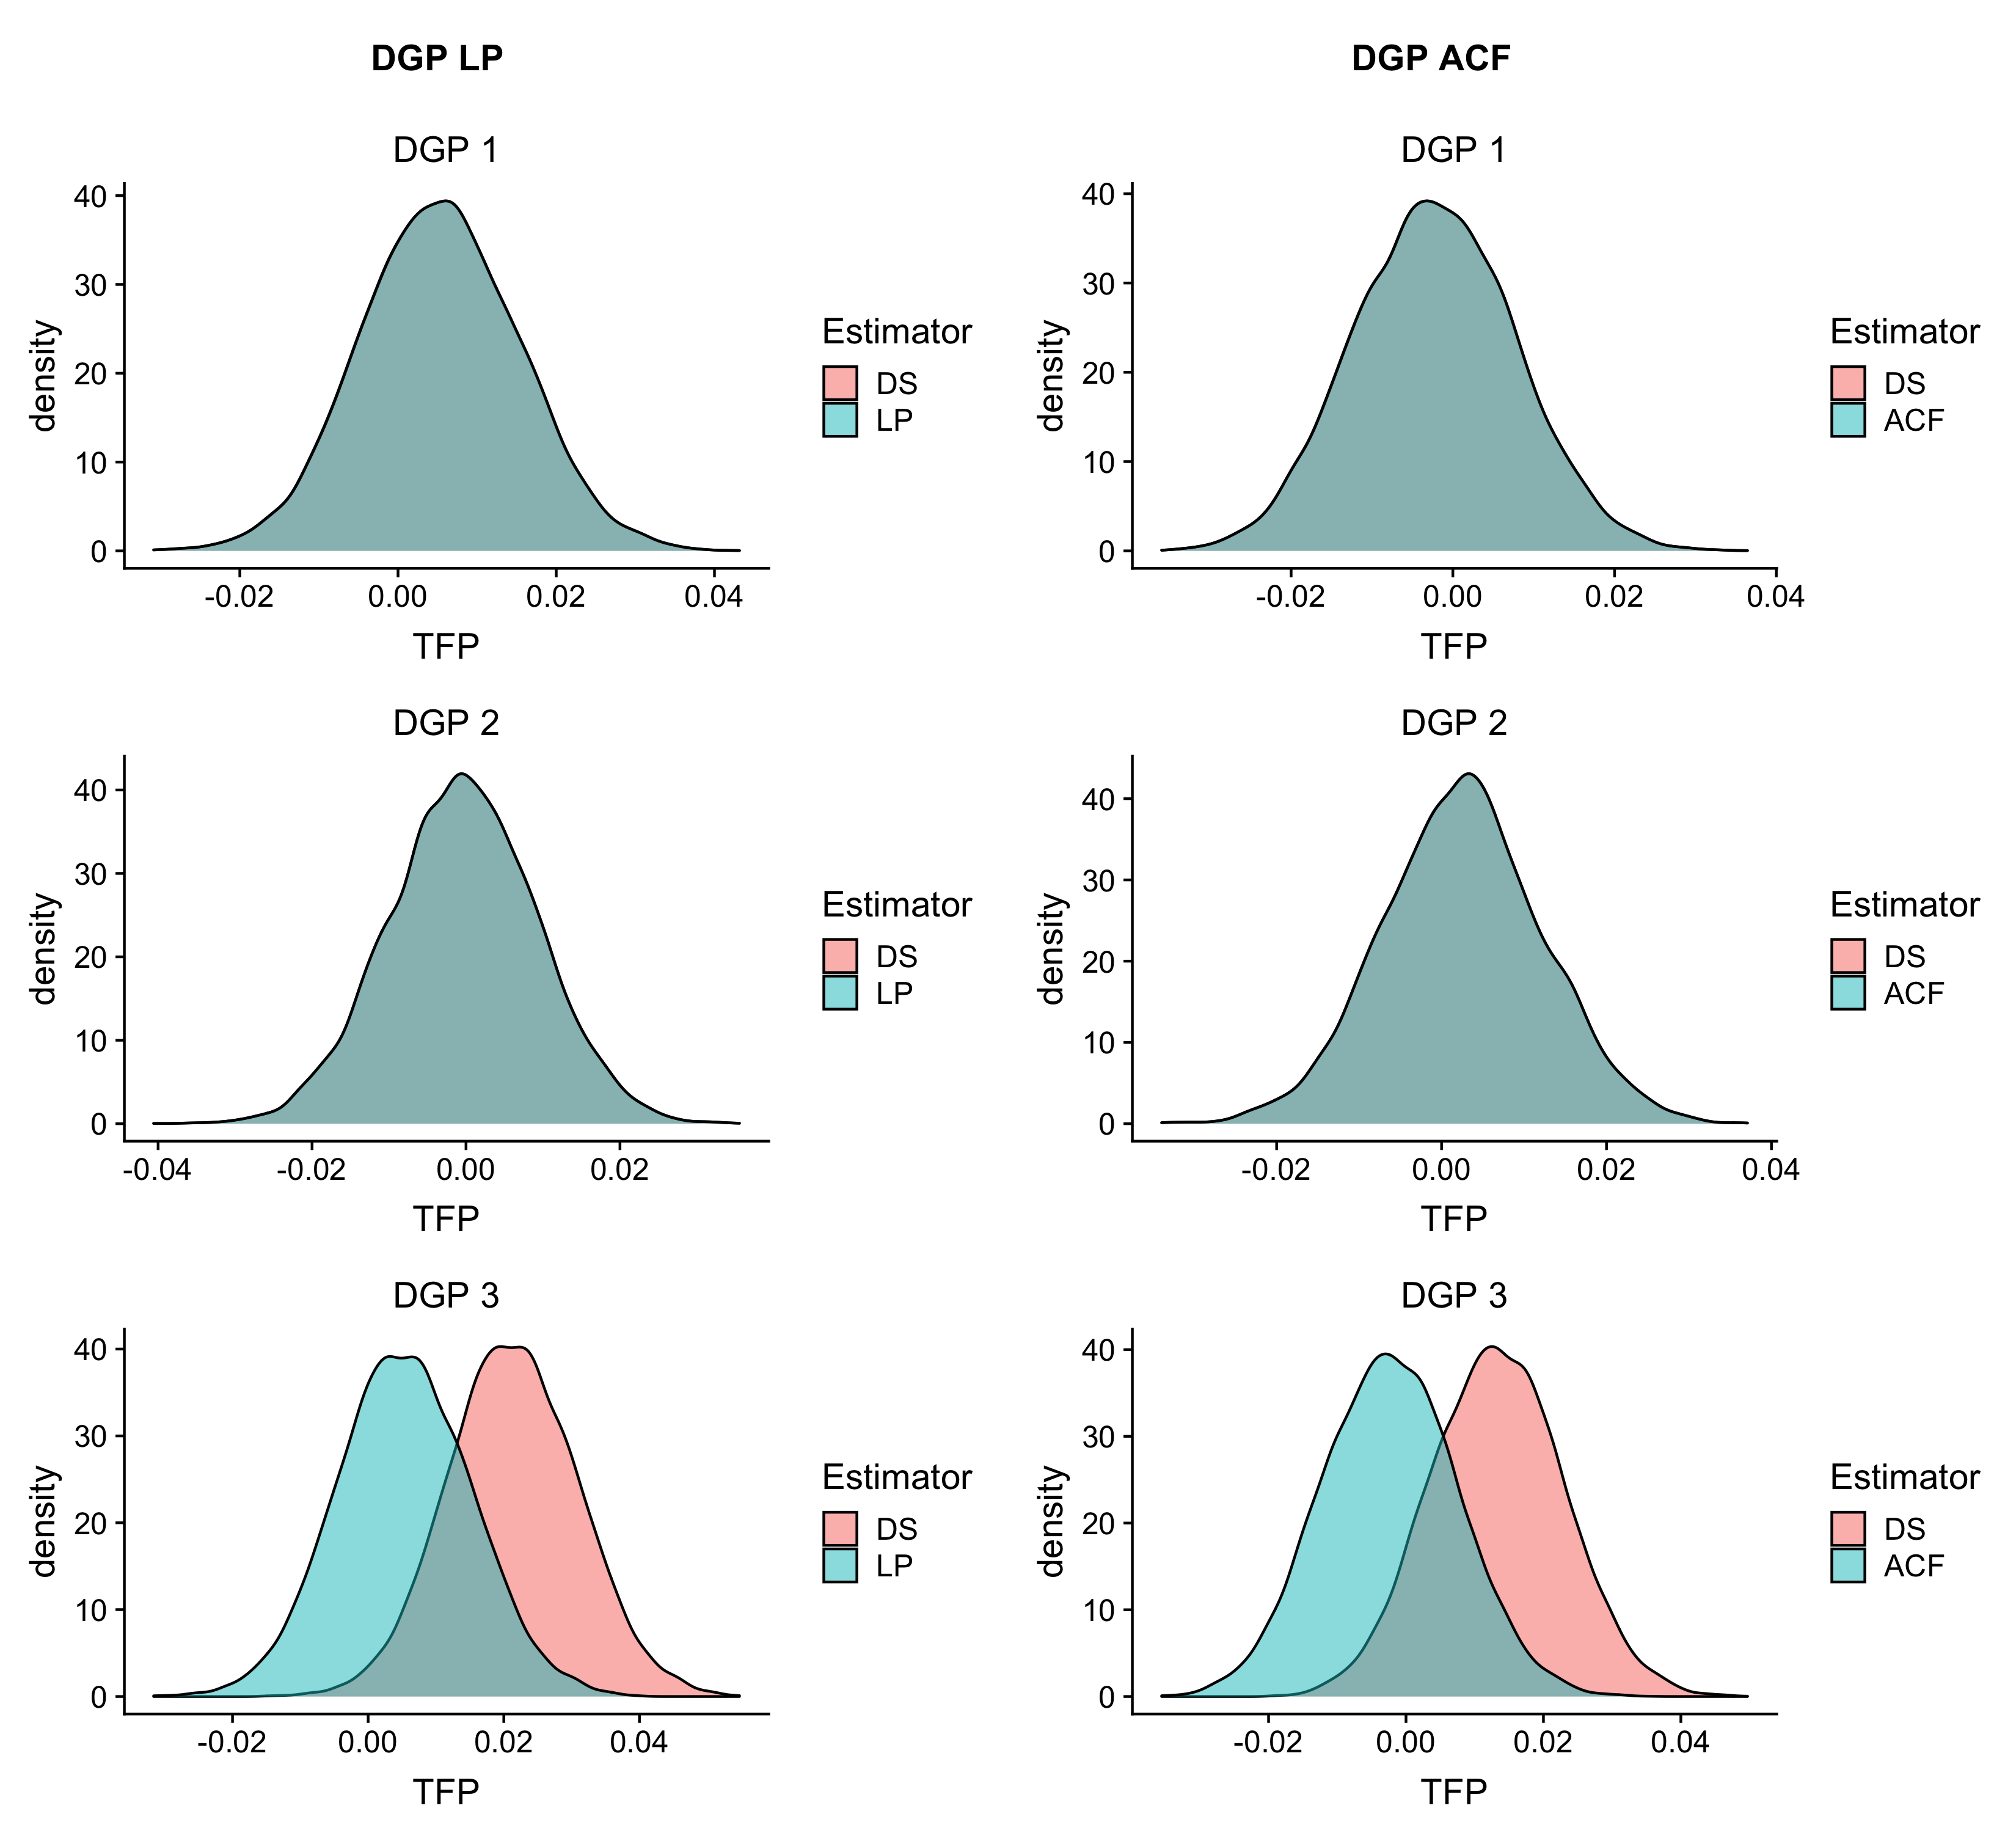
\includegraphics[width=8cm, height=5cm]{/MC/TFPplot.png}
\caption*{\footnotesize $^{*}$Estimated TFP from LP, ACF, and the median DS estimator for three DGPs: The left panel compares the LP estimator and the DS estimator when productivity is estimated using LP; The right panel compares the ACF estimator and the DS estimator when productivity is estimated using ACF.}
\label{fig:MCTFP}
\end{figure}
\end{frame}

%------------------------------------------------------------------------------------

\begin{frame}
\frametitle{Application}
\begin{itemize}
    \item Estimator is applied to firm and plant-level manufacturing datasets from US, Chile, and Colombia to examine heterogeneity in production
    \item US data comes from Compustat and covers public firms. Sample manufacturing industries from 1961 to 2016
    \item Chile data comes from the census of Chilean manufacturing plants conducted by the INE 
    \item Colombia data comes from the census of Colombian manufacturing firms conducted by the Departamenta Administrativo Nacional de Estadistica
    \item Estimates are examined across different manufacturing and industries
    \item Bootstrap to estimate standard errors of $\beta_{k}(\tau)$ and $\beta_{l}(\tau)$ with the number of iterations set to $500$.
\end{itemize}
\end{frame}

%------------------------------------------------------------------------------------

\begin{frame}
\frametitle{US Compustat}
\begin{figure}[H]
\centering
\caption{Estimated Coefficients of Capital and Labor for U.S.: NAICS 31}
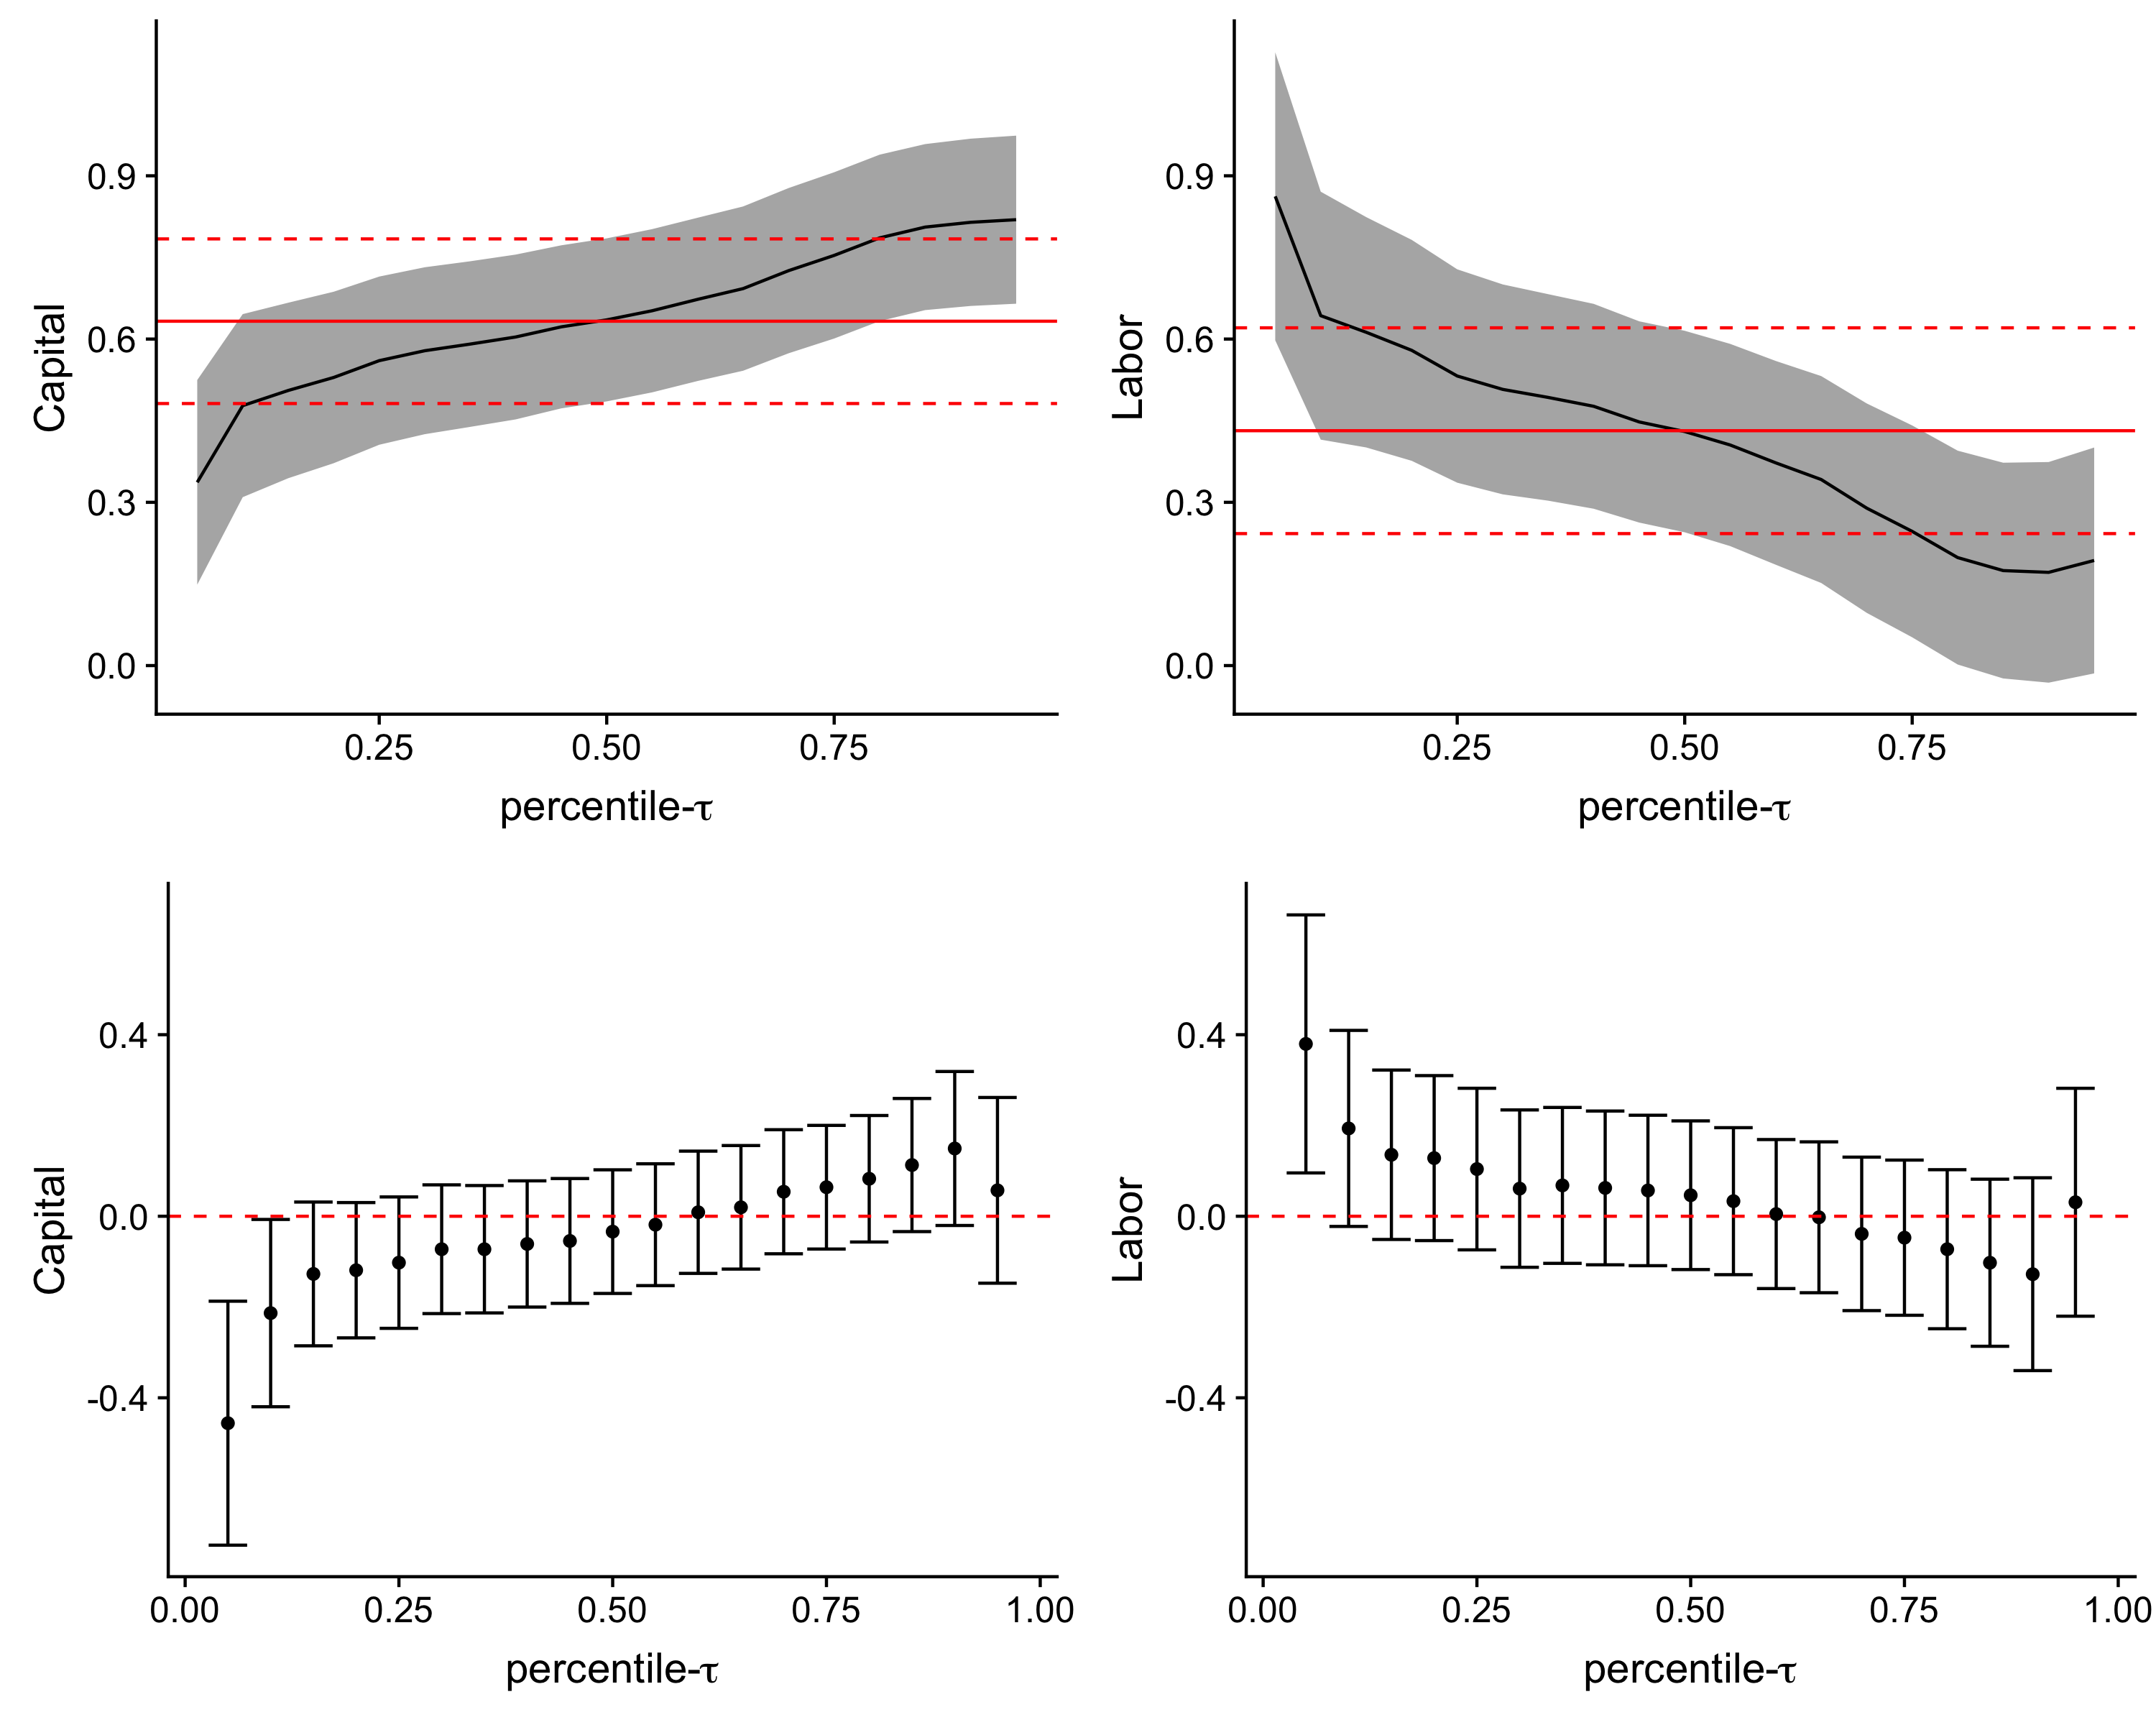
\includegraphics[width=9cm, height=5cm]{/US/QACF_Coef_Plot_NAICS_31.png}
\caption*{\footnotesize $^{*}$Top row: Estimated values of production function coefficients and their point-wise 90\% confidence interval. Bottom row: Difference between DS and QR estimates that does not control for endogeneity and their 95\% confidence intervals.}
\end{figure}
\end{frame}

%------------------------------------------------------------------------------------

\begin{frame}
\frametitle{US Compustat}
\begin{figure}[H]
\centering
\caption{Estimated Coefficients of Capital and Labor for U.S.: NAICS 32}
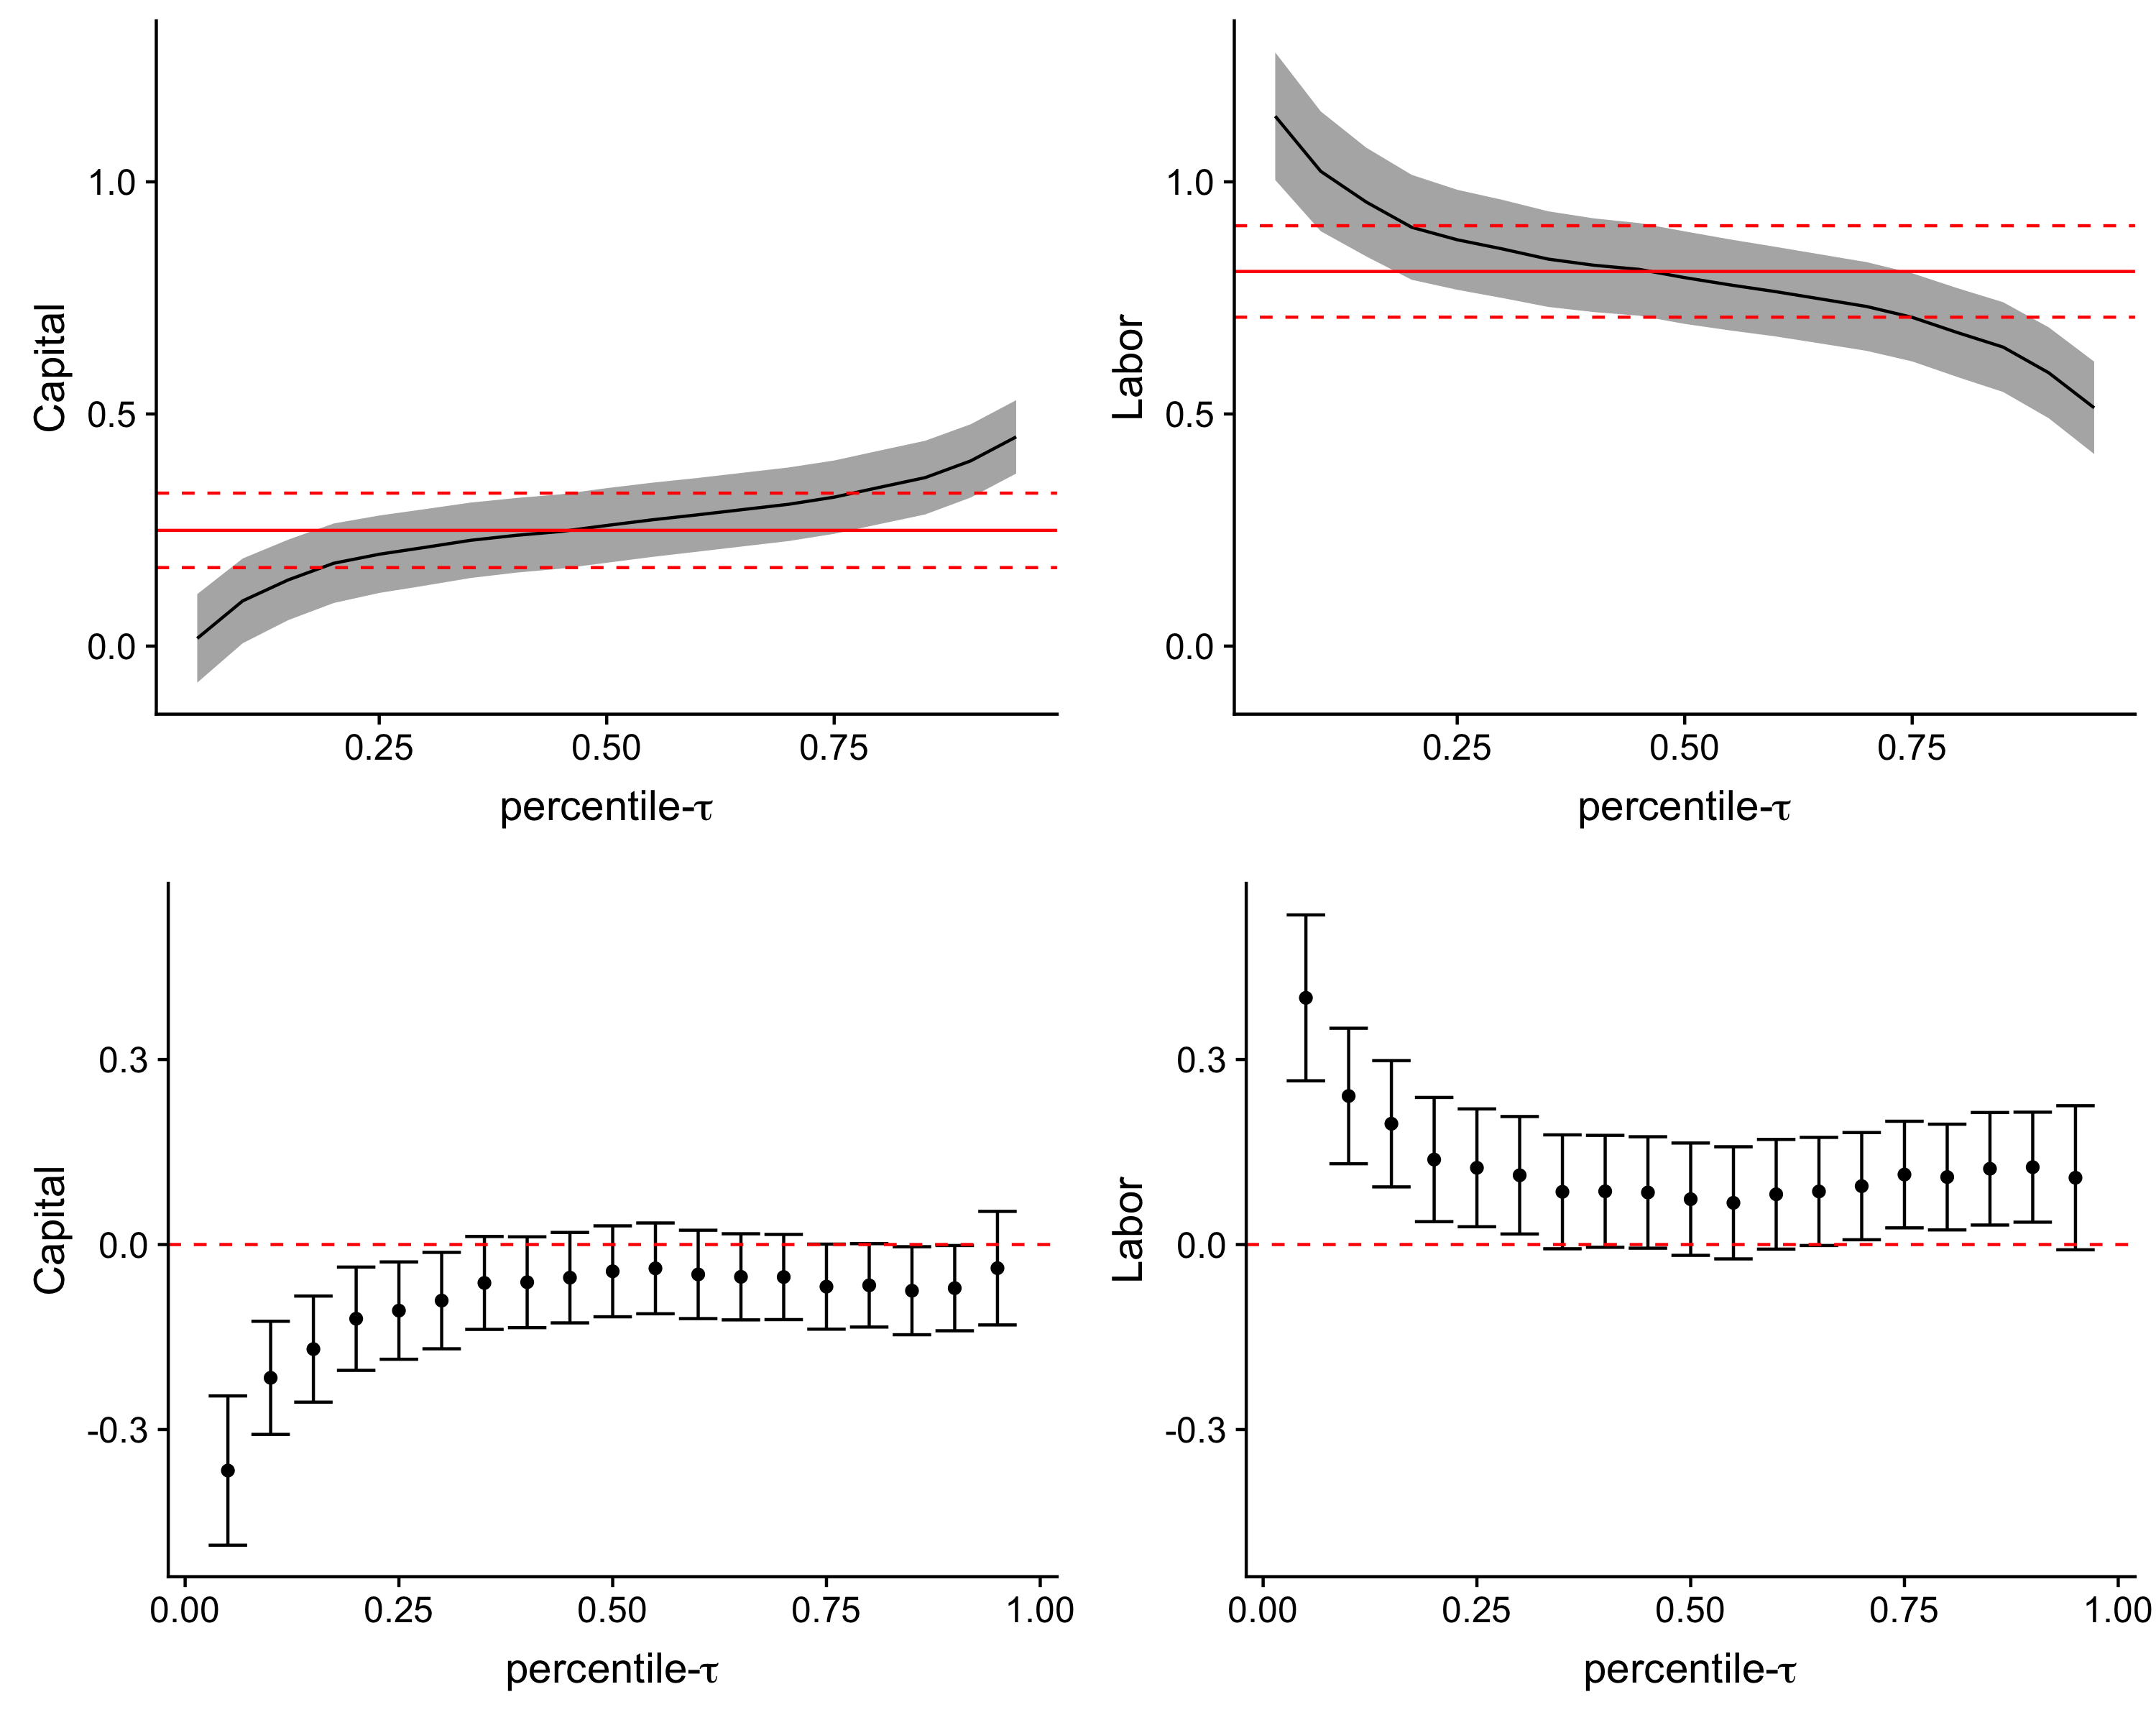
\includegraphics[width=9cm, height=5cm]{US/QACF_Coef_Plot_NAICS_32.png}
\caption*{\footnotesize $^{*}$Top row: Estimated values of production function coefficients and their point-wise 90\% confidence interval. Bottom row: Difference between DS and QR estimates that does not control for endogeneity and their 95\% confidence intervals.}
\end{figure}
\end{frame}

%------------------------------------------------------------------------------------

\begin{frame}
\frametitle{US Compustat}
\begin{figure}[H]
\centering
\caption{Estimated Coefficients of Capital and Labor for U.S.: NAICS 33}
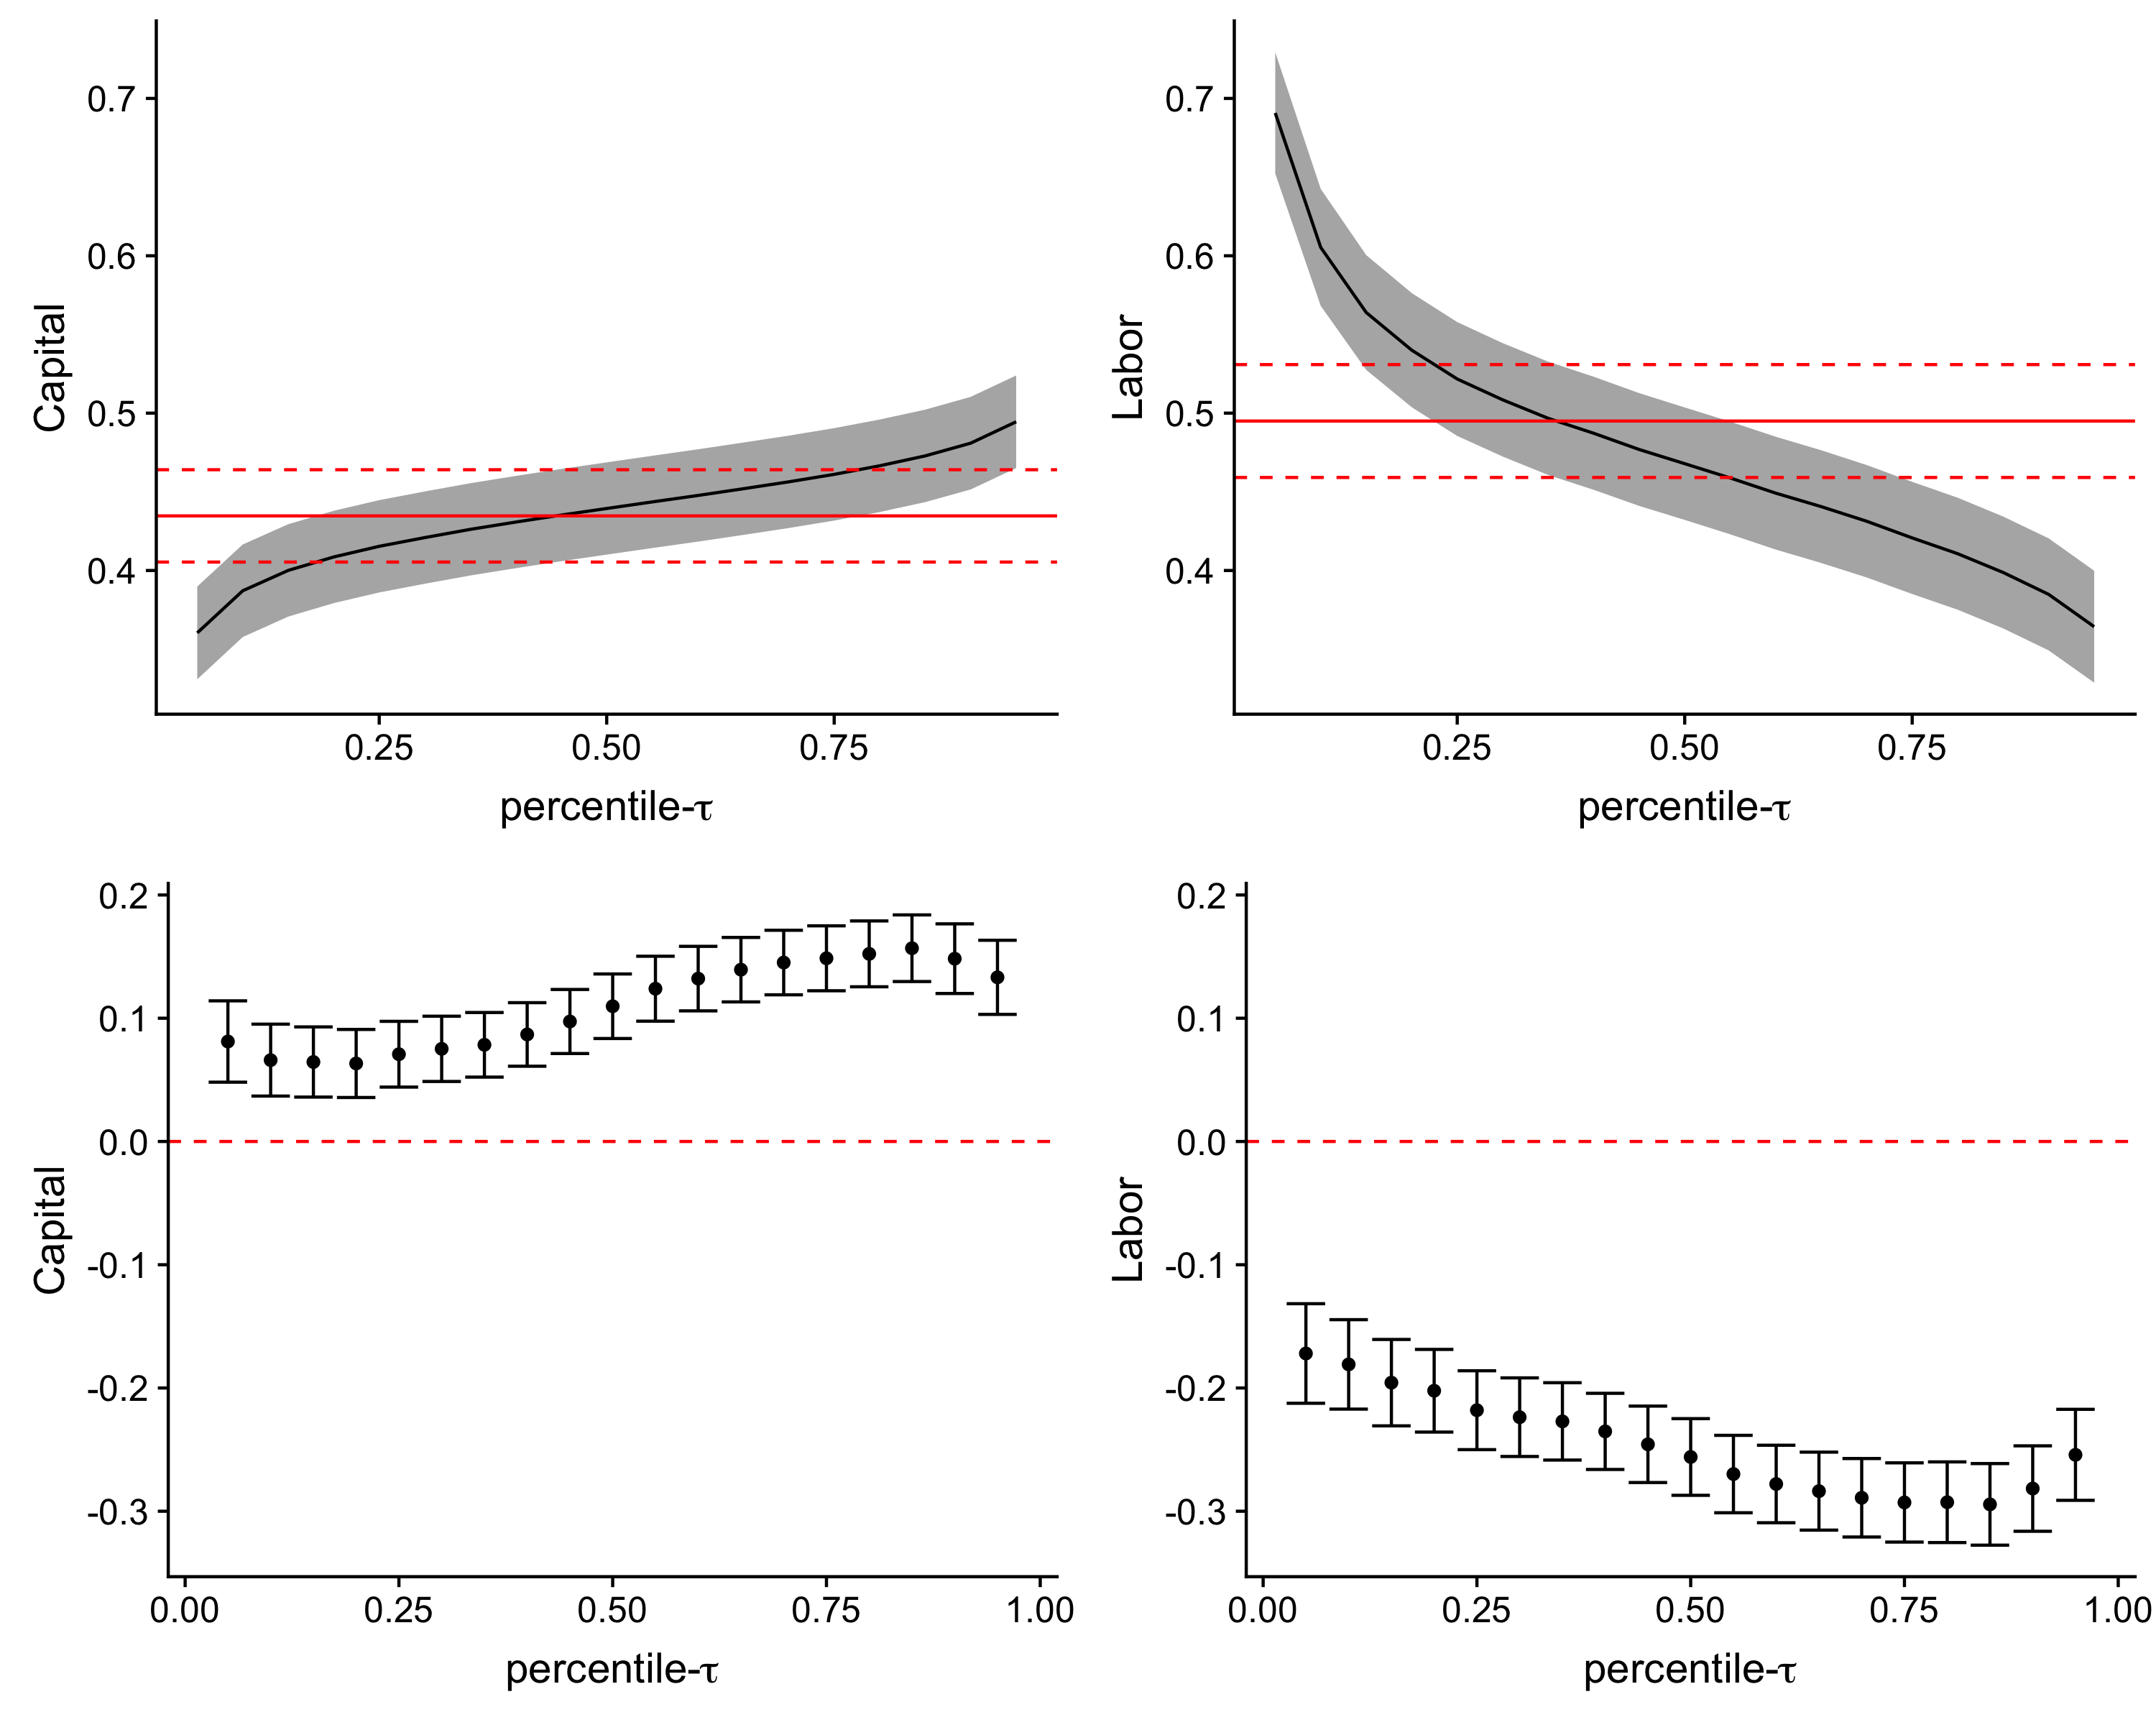
\includegraphics[width=9cm, height=5cm]{/US/QACF_Coef_Plot_NAICS_33.png}
\caption*{\footnotesize $^{*}$Top row: Estimated values of production function coefficients and their point-wise 90\% confidence interval. Bottom row: Difference between DS and QR estimates that does not control for endogeneity and their 95\% confidence intervals.}
\end{figure}
\end{frame}

%------------------------------------------------------------------------------------

\begin{frame}
\frametitle{US Compustat}
\begin{figure}[H]
\centering
\caption{Estimated Coefficients of Capital and Labor for U.S. Manufacturing Firms}
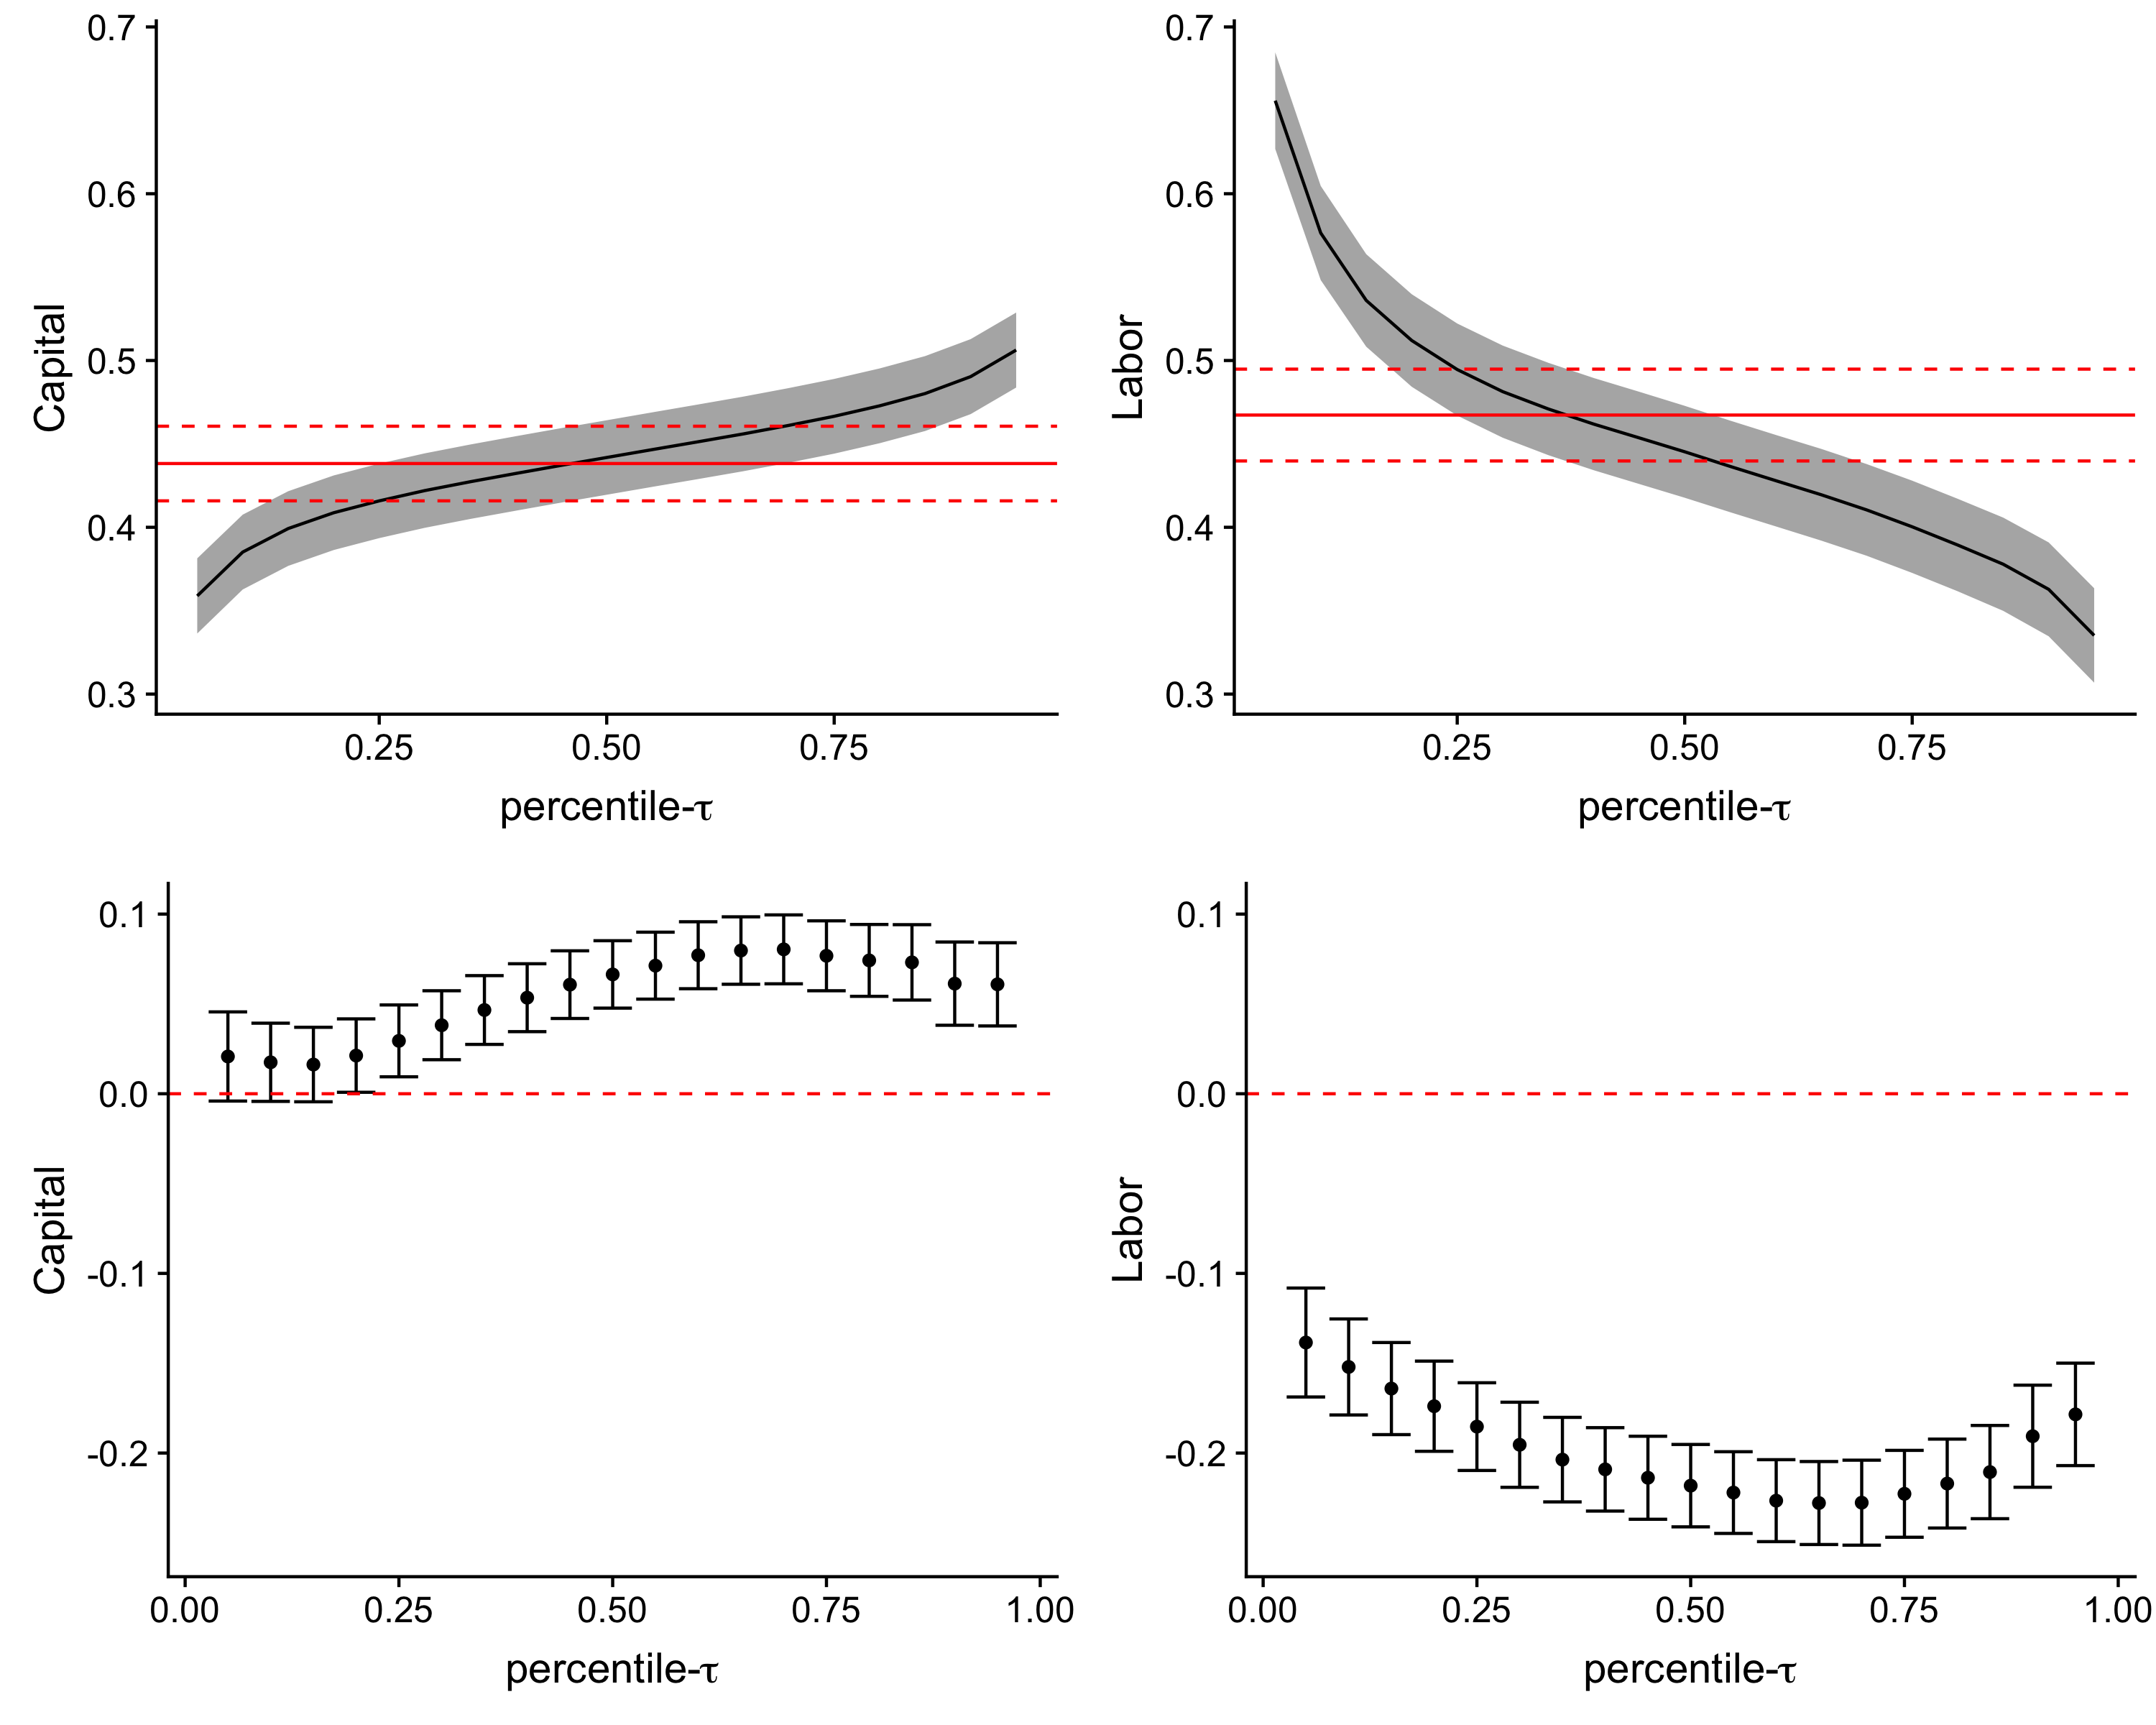
\includegraphics[width=9cm, height=5cm]{/US/QACF_Coef_Plot_NAICS_All.png}
\caption*{\footnotesize $^{*}$Top row: Estimated values of production function coefficients and their point-wise 90\% confidence interval. Bottom row: Difference between DS and QR estimates that does not control for endogeneity and their 95\% confidence intervals.}
\end{figure}
\end{frame}

%------------------------------------------------------------------------------------

\begin{frame}
\frametitle{US Compustat}
\resizebox{\linewidth}{!}{
\begin{tabular}{cccccccccc}
  \hline\hline & & \multicolumn{2}{c}{Capital}  & \multicolumn{2}{c}{Labor} & \multicolumn{2}{c}{Returns to Scale} & \multicolumn{2}{c}{Capital Intensity}\\ \cmidrule(lr){3-4} \cmidrule(lr){5-6} \cmidrule(lr){7-8} \cmidrule(lr){9-10}NAICS & $\tau$ & Coef. & s.e & Coef. & s.e & Coef. & s.e & Coef. & s.e \\ 
  \hline
31 & 0.10 & 0.319 & 0.0323 & 0.554 & 0.0383 & 0.873 & 0.0161 & 0.575 & 0.0787 \\ 
   & 0.25 & 0.345 & 0.0324 & 0.500 & 0.0375 & 0.845 & 0.0143 & 0.689 & 0.0915 \\ 
   & 0.50 & 0.372 & 0.0323 & 0.450 & 0.0369 & 0.821 & 0.0133 & 0.827 & 0.1073 \\ 
   & 0.90 & 0.422 & 0.0327 & 0.374 & 0.0390 & 0.797 & 0.0204 & 1.127 & 0.1420 \\ 
  32 & 0.10 & 0.189 & 0.0280 & 0.766 & 0.0359 & 0.955 & 0.0132 & 0.246 & 0.0478 \\ 
   & 0.25 & 0.217 & 0.0279 & 0.692 & 0.0349 & 0.909 & 0.0119 & 0.313 & 0.0555 \\ 
   & 0.50 & 0.242 & 0.0279 & 0.639 & 0.0346 & 0.881 & 0.0114 & 0.378 & 0.0630 \\ 
   & 0.90 & 0.293 & 0.0278 & 0.540 & 0.0354 & 0.833 & 0.0127 & 0.543 & 0.0835 \\ 
  33 & 0.10 & 0.387 & 0.0179 & 0.605 & 0.0226 & 0.992 & 0.0070 & 0.640 & 0.0283 \\ 
   & 0.25 & 0.415 & 0.0178 & 0.522 & 0.0220 & 0.937 & 0.0061 & 0.796 & 0.0330 \\ 
   & 0.50 & 0.439 & 0.0178 & 0.468 & 0.0217 & 0.907 & 0.0058 & 0.939 & 0.0371 \\ 
   & 0.90 & 0.481 & 0.0179 & 0.385 & 0.0216 & 0.866 & 0.0057 & 1.250 & 0.0459 \\ 
  All & 0.10 & 0.385 & 0.0136 & 0.576 & 0.0172 & 0.962 & 0.0055 & 0.668 & 0.0262 \\ 
   & 0.25 & 0.416 & 0.0136 & 0.495 & 0.0168 & 0.910 & 0.0049 & 0.841 & 0.0311 \\ 
   & 0.50 & 0.442 & 0.0136 & 0.445 & 0.0168 & 0.887 & 0.0052 & 0.992 & 0.0354 \\ 
   & 0.90 & 0.490 & 0.0137 & 0.363 & 0.0171 & 0.853 & 0.0064 & 1.352 & 0.0458 \\  
   \hline
\end{tabular}}
\end{frame}

%------------------------------------------------------------------------------------

\begin{frame}
\frametitle{US Compustat}
\begin{figure}[H]
\centering
\caption{DS and ACF Estimates of Log Total Factor Productivity}
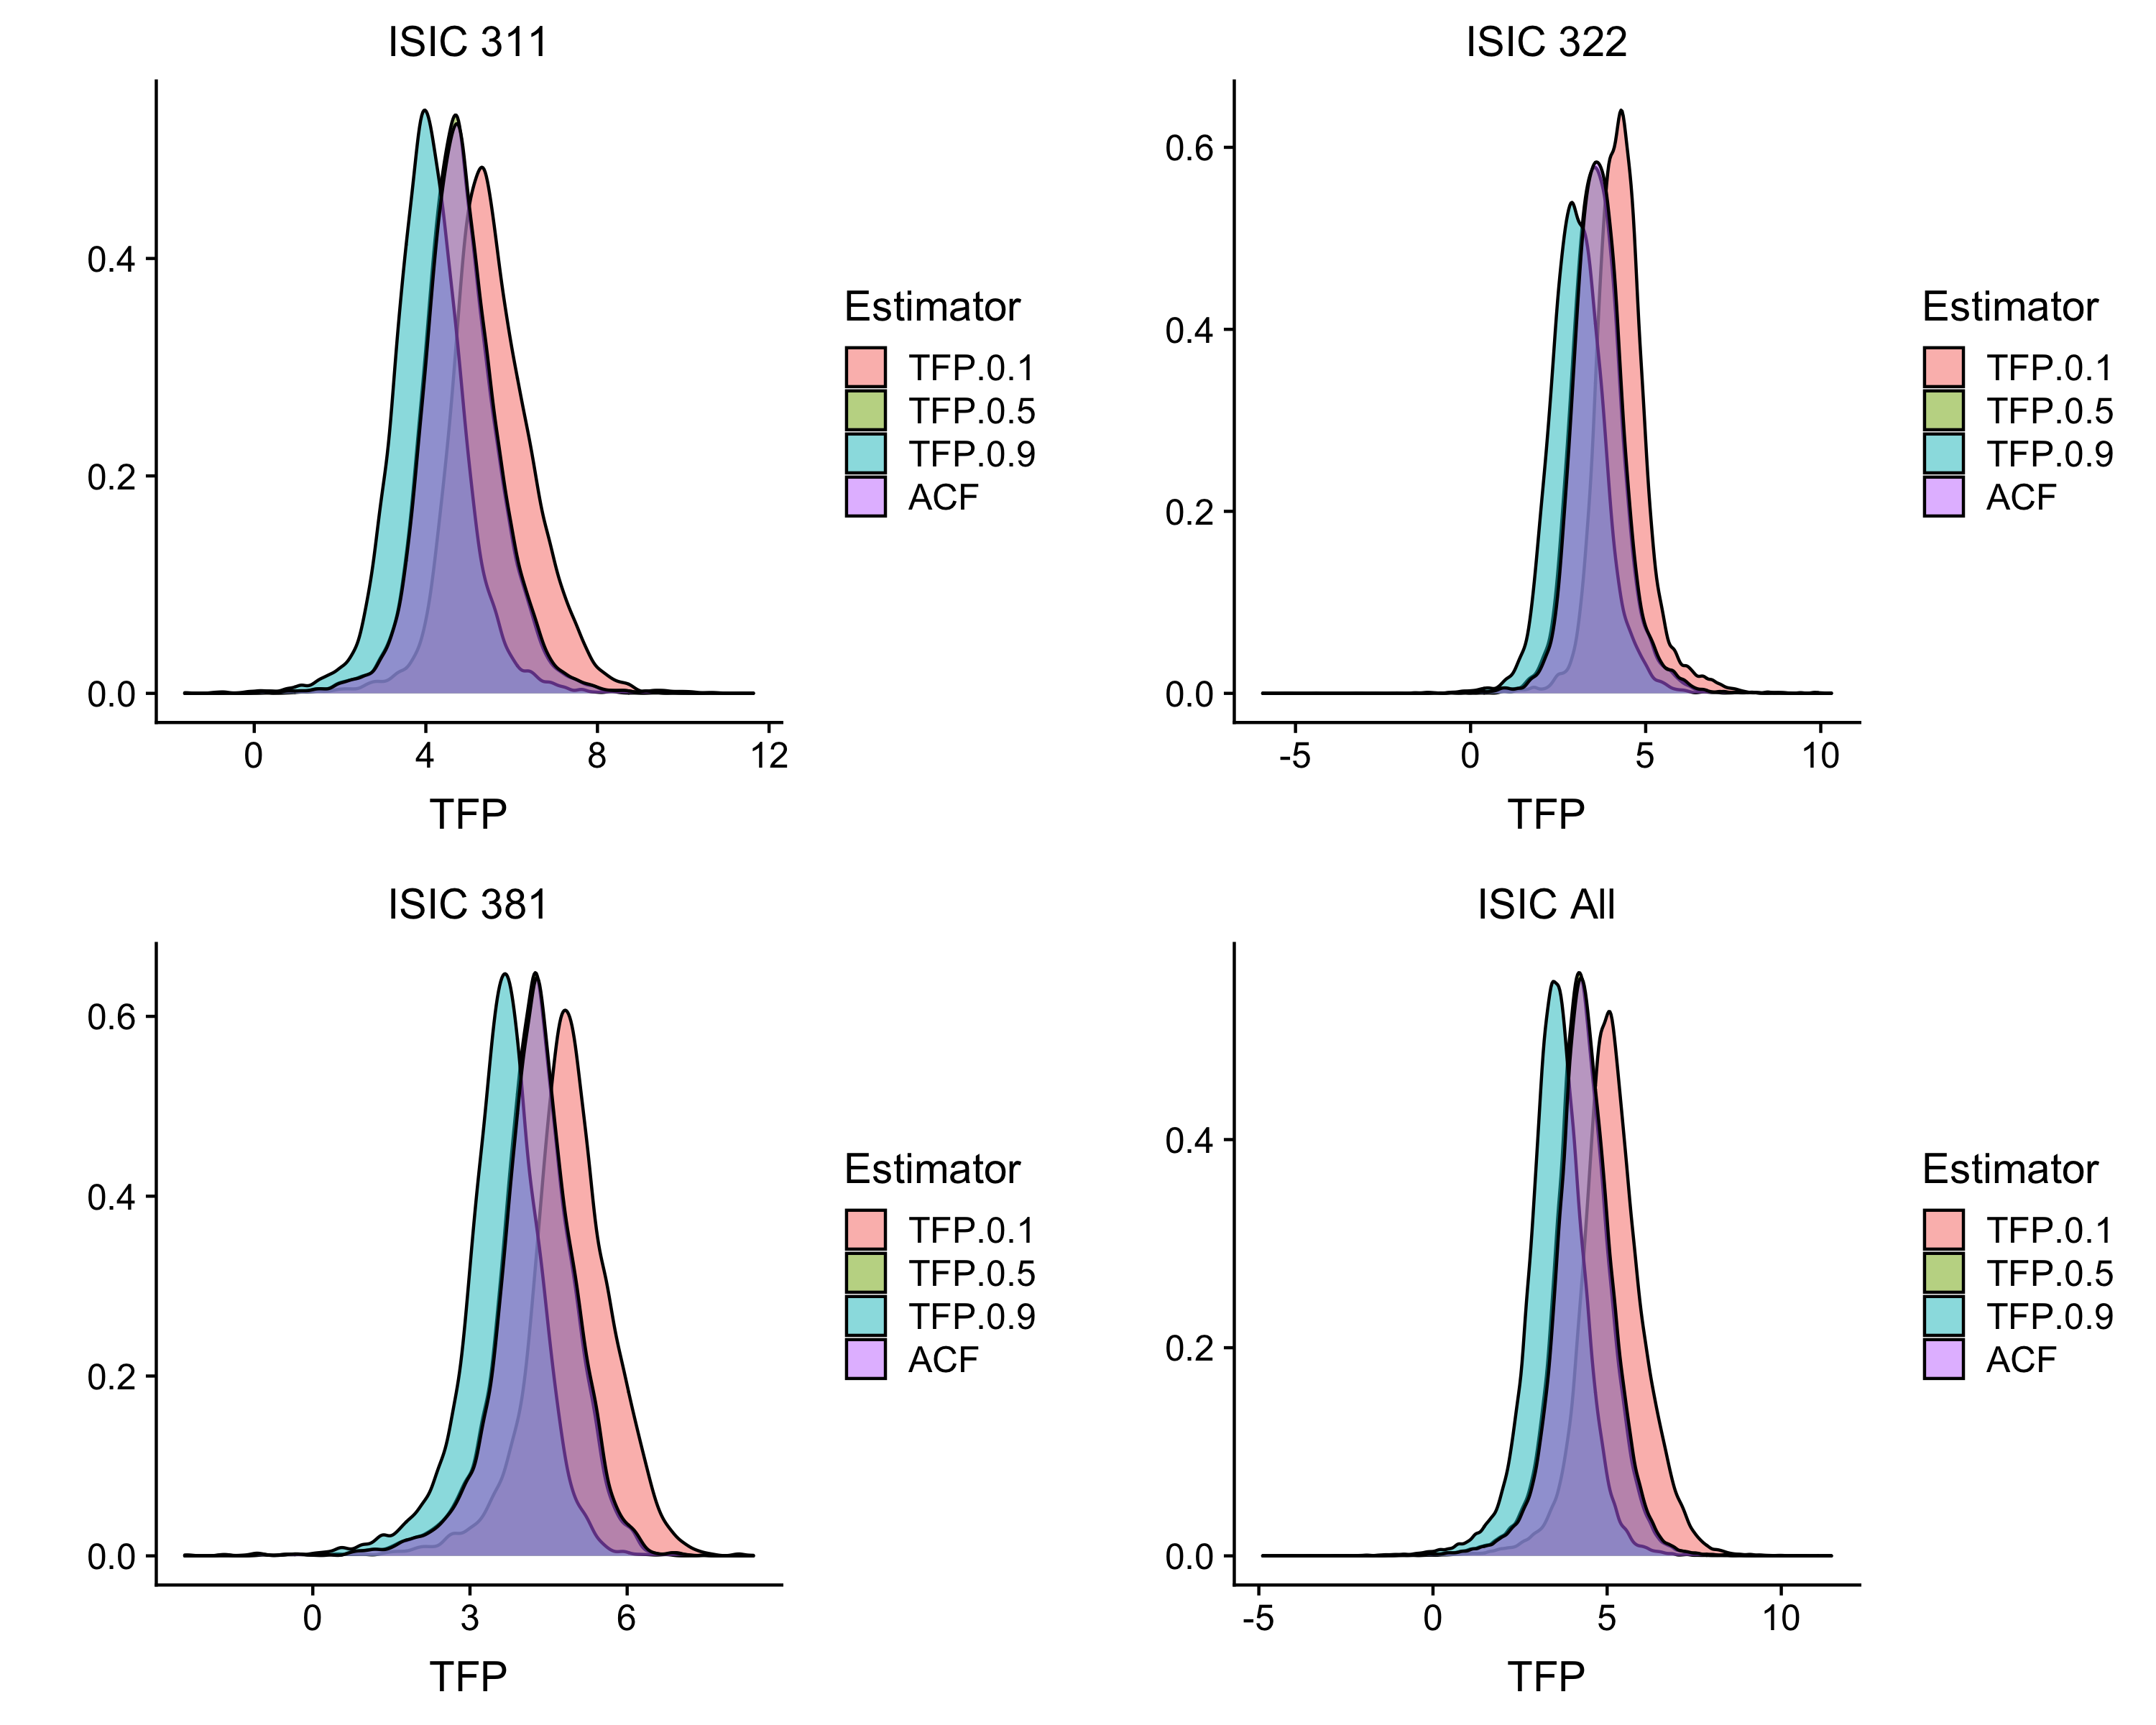
\includegraphics[width=9cm, height=5cm]{/US/QACF_TFP_Plot.png}
\caption*{\footnotesize $^{*}$Estimated Distributions of TFP from the DS estimator for $\tau \in \{0.1, 0.5, 0.9\}$ and those from  the ACF estimator.}
\label{fig:QACFUSTFP}
\end{figure}
\end{frame}

%------------------------------------------------------------------------------------

\begin{frame}
\frametitle{US Compustat}
\begin{figure}[H]
\centering
\caption{U.S. Productivity Over Time}
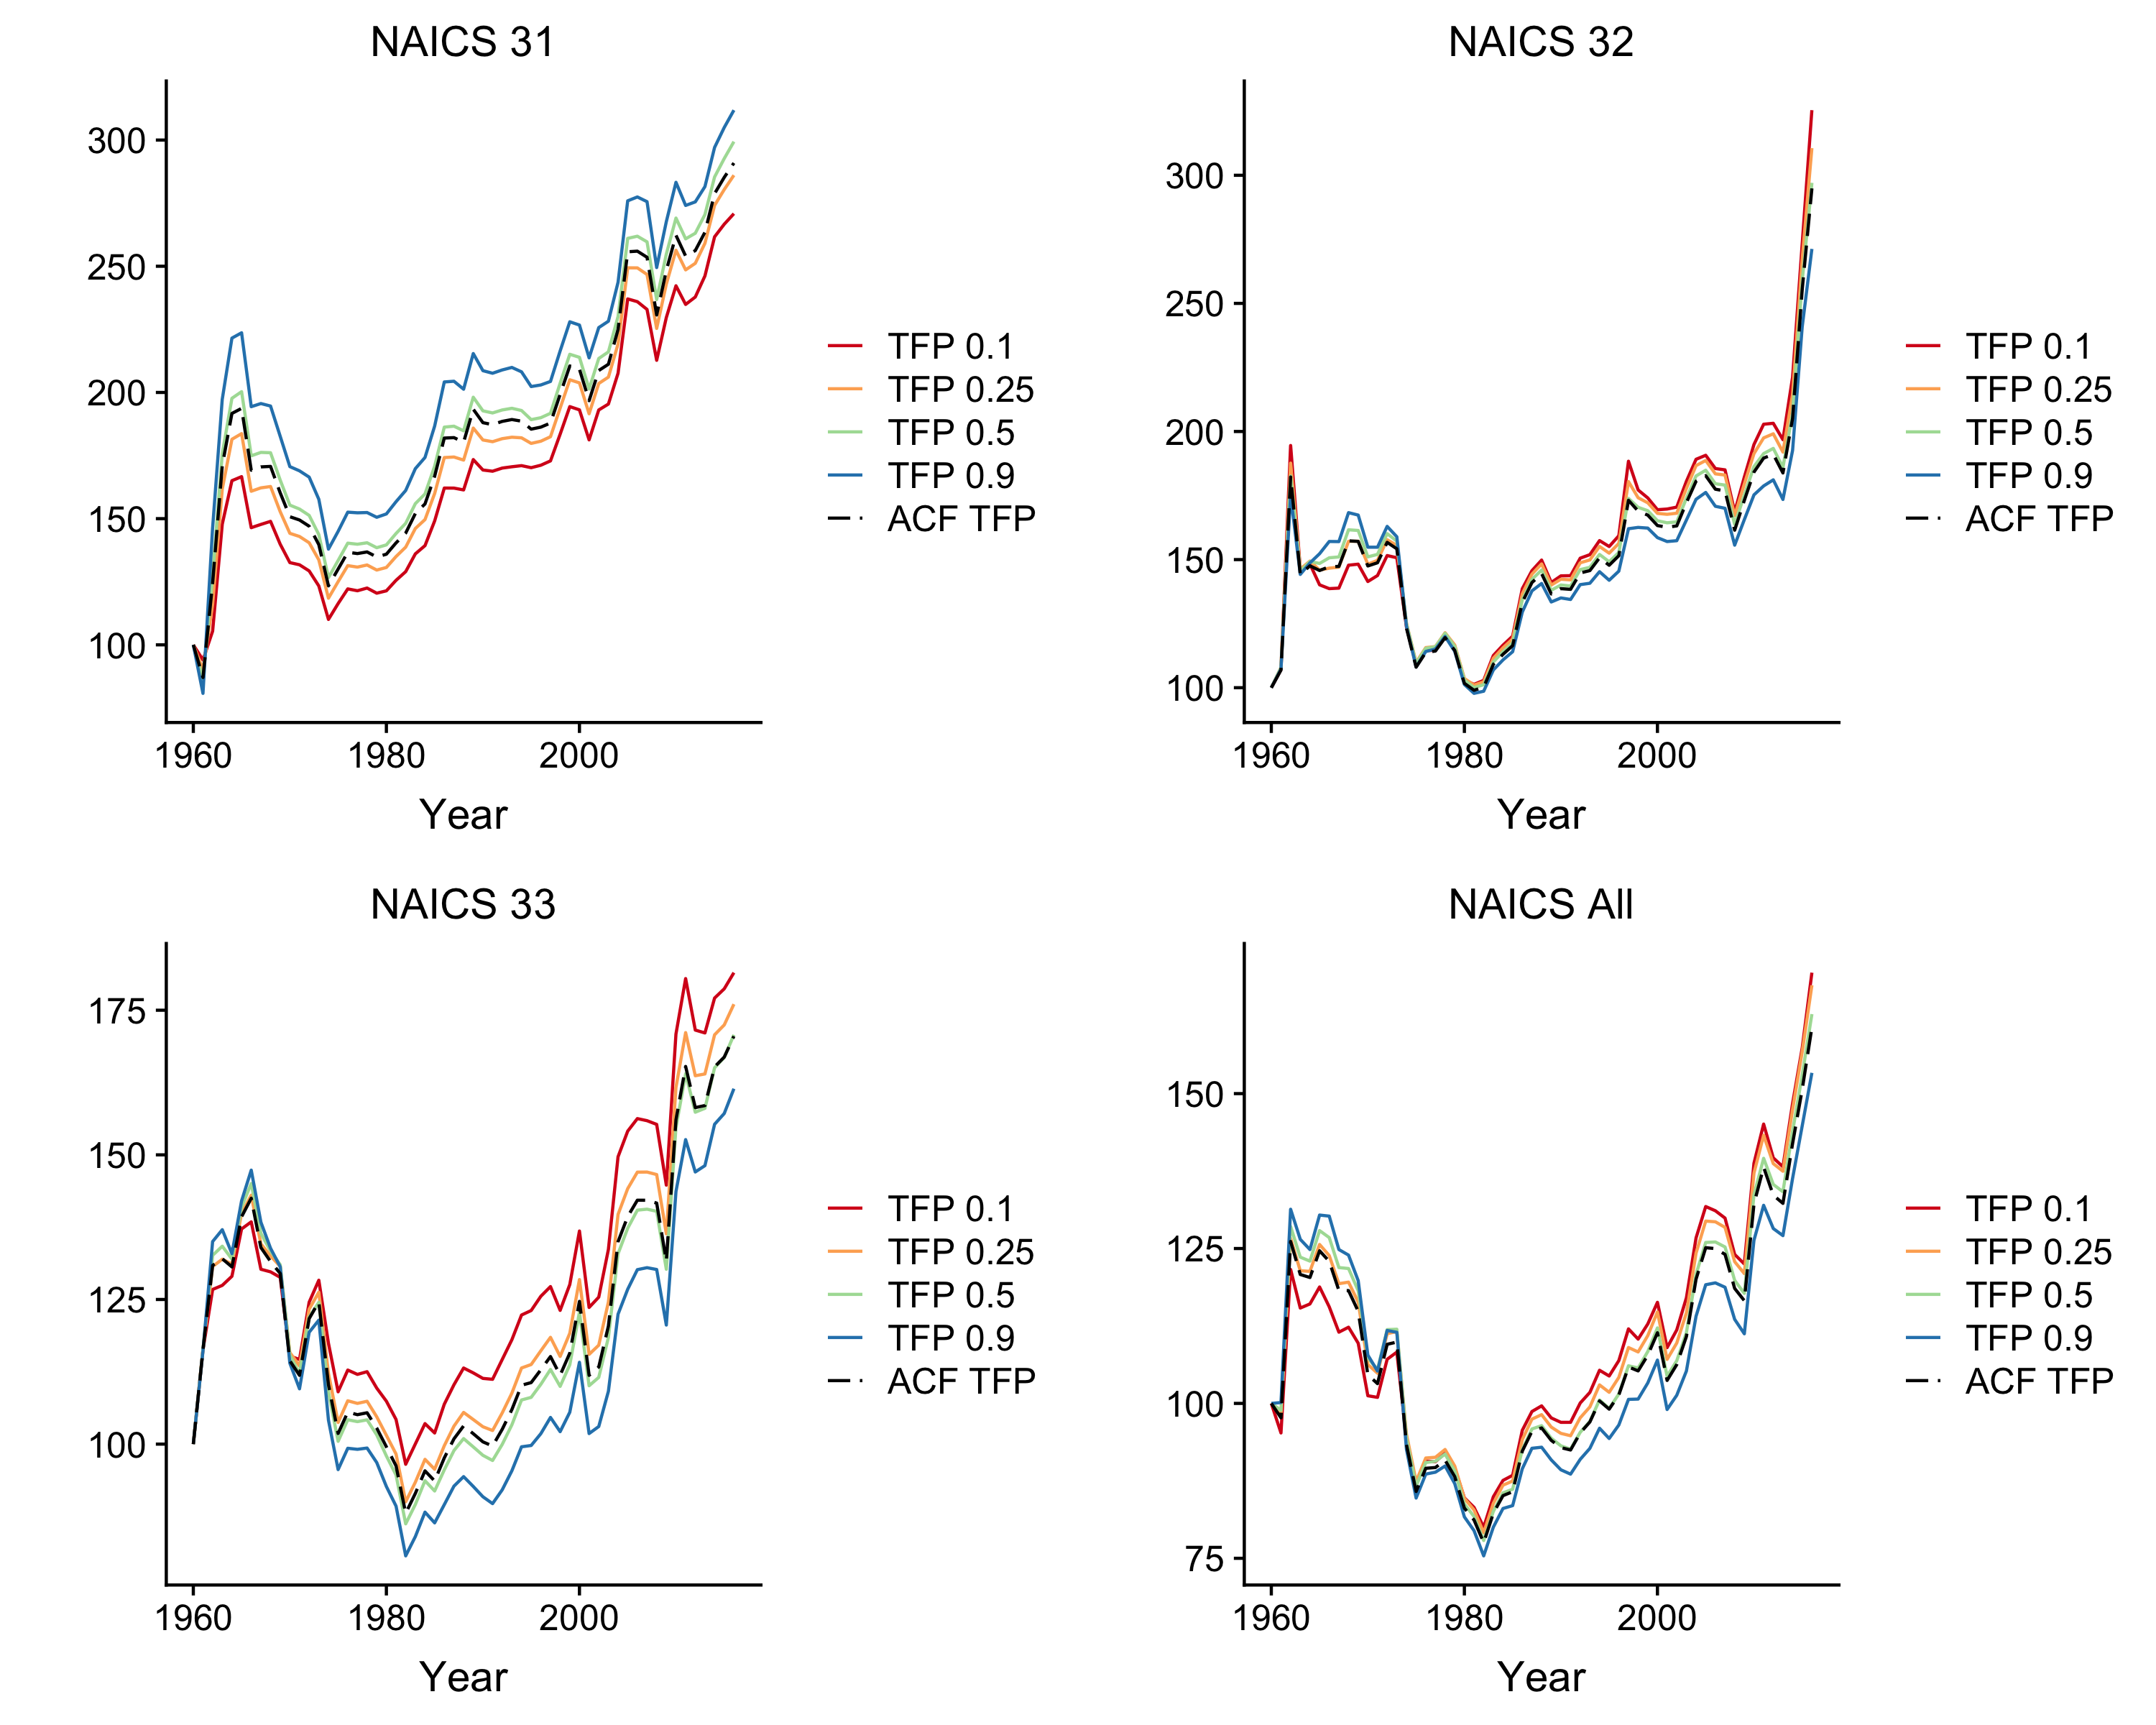
\includegraphics[width=9cm, height=5cm]{/US/QACF_TFPgrowth_Plot.png}
\caption*{\footnotesize $^{*}$Estimated average productivity (in levels) over time for the U.S. Base year productivity is set to 100.}
\label{fig:QACFUSTFPG}
\end{figure}
\end{frame}

%------------------------------------------------------------------------------------

\begin{frame}
\frametitle{US Compustat}
\small
\centering
\begin{tabular}{cccccccccc}
  \hline\hline & & \multicolumn{2}{c}{R\&D}  & \multicolumn{2}{c}{Advertisements} \\ \cmidrule(lr){3-4} \cmidrule(lr){5-6}NAICS & $\tau$ & Coef. & s.e & Coef. & s.e \\ 
  \hline
31 & 0.10 & 0.157 & 0.0160 & 0.187 & 0.0197 \\ 
   & 0.25 & 0.170 & 0.0143 & 0.200 & 0.0178 \\ 
   & 0.50 & 0.181 & 0.0133 & 0.211 & 0.0162 \\ 
   & 0.90 & 0.190 & 0.0139 & 0.219 & 0.0159 \\ 
  32 & 0.10 & 0.105 & 0.0092 & 0.112 & 0.0105 \\ 
   & 0.25 & 0.133 & 0.0093 & 0.139 & 0.0103 \\ 
   & 0.50 & 0.148 & 0.0088 & 0.154 & 0.0098 \\ 
   & 0.90 & 0.175 & 0.0088 & 0.180 & 0.0099 \\ 
  33 & 0.10 & 0.064 & 0.0054 & 0.048 & 0.0054 \\ 
   & 0.25 & 0.098 & 0.0047 & 0.076 & 0.0047 \\ 
   & 0.50 & 0.115 & 0.0046 & 0.091 & 0.0045 \\ 
   & 0.90 & 0.138 & 0.0050 & 0.109 & 0.0047 \\ 
  All & 0.10 & 0.097 & 0.0047 & 0.082 & 0.0051 \\ 
   & 0.25 & 0.126 & 0.0042 & 0.109 & 0.0045 \\ 
   & 0.50 & 0.138 & 0.0040 & 0.120 & 0.0043 \\ 
   & 0.90 & 0.154 & 0.0042 & 0.133 & 0.0042 \\ 
   \hline
\end{tabular}
\end{frame}

%------------------------------------------------------------------------------------

\begin{frame}
\frametitle{Conclusion}
\begin{itemize}
	\item Proposed a method that extends the control function approach to quantiles of firm output
	\item Computationally attractive, easy to implement
	\item Estimator works well in finite samples, consistent and asymptotically normal
	\item Limitations of control function approach apply to this model as well
	\item Future work could find the extension to gross-output production function in the framework of \cite{Gandhi2020}
	\item Allowing for richer distributional effects: in productivity and inputs is desirable
\end{itemize}
\end{frame}


% \begin{frame}
% \frametitle{References}
% \printbibliography
% \end{frame}



\end{document}

